% ----------- Cover Master Thesis Faculty of Sciences ---------------
% This document should be compiled with pdflatex.  If you want to use
% latex to compile to dvi/ps, you have to convert the images to (e)ps
%                           -- December 2012
% -------------------------------------------------------------------
\RequirePackage{fix-cm}
\documentclass[12pt,a4paper,oneside]{book}

% ------------------------- Load packages ---------------------------
% You can eventually add these while you load other packages
% in case you want to integrate the titlepage with the rest of your thesis
% -------------------------------------------------------------------
\usepackage{graphicx,xcolor,textpos}


\renewcommand{\familydefault}{\sfdefault} % one could turn off this one
\usepackage{helvet}                       % one could turn off this one
%\usepackage[scaled=0.92]{helvet}
%\usepackage[scaled=1]{newtxsf}
\usepackage[helvet]{sfmath}               % one could turn off this one
%\usepackage{cmbright}
\usepackage{amsmath, amsfonts, amssymb}
\usepackage{booktabs}
%\usepackage[style = chem-acs]{biblatex}
\usepackage[numbers,sort&compress]{natbib}
\usepackage{siunitx}
\usepackage{subcaption}
\usepackage{svg}
\usepackage[T1]{fontenc}
\usepackage{setspace}
%\usepackage[nottoc,numbib]{tocbibind}
\usepackage{algorithm}
\usepackage{algpseudocode}

\usepackage{longtable} % For tables that span multiple pages
\usepackage{array}     % For advanced column formatting (like p{})
\newcolumntype{L}[1]{>{\raggedright\arraybackslash}p{#1}}
\usepackage{pdflscape} % For landscape pages

\usepackage[font=small]{caption}

\usepackage{hyperref}

% ------------------------ Page settings -----------------------------
% If you change these, the cover layout will also change.  In that
% case you have to adjust the latter manually.
% --------------------------------------------------------------------

\topmargin -10mm
\textwidth 160truemm
\textheight 240truemm
\oddsidemargin 0mm
\evensidemargin 0mm

% ---------------------- textpos settings ----------------------------
% Some additional settings for the cover
% --------------------------------------------------------------------

\definecolor{green}{RGB}{172,196,0}
\definecolor{bluetitle}{RGB}{29,141,176}
\definecolor{blueaff}{RGB}{0,0,128}
\definecolor{blueline}{RGB}{82,189,236}
\setlength{\TPHorizModule}{1mm}
\setlength{\TPVertModule}{1mm}

\begin{document}

% ----------------------- Cover --------------------------------------
% Please fill in:
% - The title and subtitle (if applicable)
%         to include a formula in the title or subtitle
%         use  \form{$...$}
% - Your name
% - Your (co)supervisor, mentor (if applicable)
% - Your master
% - The academic year
% --------------------------------------------------------------------
\thispagestyle{empty}
\newcommand{\form}[1]{\scalebox{1.087}{\boldmath{#1}}}
\sffamily % one could change this one to 'rmfamily'
%
\begin{textblock}{191}(-24,-11)
\colorbox{bluetitle}{\hspace{139mm}\ \parbox[c][18truemm]{52mm}{\textcolor{white}{FACULTY OF SCIENCE}}}
\end{textblock}
%
\begin{textblock}{70}(-18,-19)
\textblockcolour{}
\includegraphics*[height=19.8truemm]{LogoKULeuven}
\end{textblock}
%
\begin{textblock}{160}(-6,63)
\textblockcolour{}
\vspace{-\parskip}
\flushleft
\fontsize{35}{37}\selectfont \textcolor{bluetitle}{\textit{Ab Initio} Molecular Dynamics Simulations of Phosphate Hydrolysis Using Neural Network Potentials}\\[1.5mm]
%\fontsize{20}{22}\selectfont Dynamics and Reactivity
\end{textblock}
%
\begin{textblock}{160}(8,153)
\textblockcolour{}
\vspace{-\parskip}
\flushright
\fontsize{14}{16}\selectfont \textbf{Albert MAKHMUDOV}
\end{textblock}
%
\begin{textblock}{70}(-6,191)
\textblockcolour{}
\vspace{-\parskip}
\flushleft
Supervisor: Prof. J. Harvey\\[-2pt]
\textcolor{blueaff}{KU Leuven}\\[5pt]
%Mentor: Prof. J. Harvey\\[-2pt]
%\textcolor{blueaff}{KU Leuven}\\
\end{textblock}
%
\begin{textblock}{160}(8,191)
\textblockcolour{}
\vspace{-\parskip}
\flushright
Thesis presented in\\[4.5pt]
fulfillment of the requirements\\[4.5pt]
for the degree of Master of Science\\[4.5pt]
in Theoretical Chemistry and Computational Modelling\\
\end{textblock}
%
\begin{textblock}{160}(8,232)
\textblockcolour{}
\vspace{-\parskip}
\flushright
Academic year 2024-2025
\end{textblock}
%
\begin{textblock}{191}(-24,248)
{\color{blueline}\rule{550pt}{5.5pt}}
\end{textblock}
%


% In case you want to integrate the TeX-file for the titlepage
% with the rest of your thesis, you cab continue below
% ------------------------- First pages ---------------------------
% For table of contents, acknowlegments, ...
% -----------------------------------------------------------------
%\rmfamily
\setcounter{page}{0}
\pagenumbering{roman}
\onehalfspacing

\include{copyright}
\chapter*{Foreword}  
% This thesis provided me with the opportunity to apply the theory and methods I acquired throughout the entire master's programme to the study of enzymatic processes, aligning perfectly with my interest in biological systems. The research was conducted in collaboration with the research group led by Prof. Iñaki Tuñón at the University of Valencia, well known for their expertise in modelling enzymatic reactions. 
% \par\bigskip
% \noindent I would like to express my gratitude to both Prof. Jeremy Harvey and Prof. Iñaki Tuñón for giving me the opportunity to independently explore my ideas as well as providing invaluable assistance and guidance whenever needed. Their kind and friendly attitude ensured that this whole project was a very enjoyable experience for me.
% \par\bigskip
% \noindent Thanks to all members of the ``Modeling Chemical Processes in Biological Environments'' research group, as well as to TCCM students in Valencia, for their openness and friendliness which made my stay in Valencia feel like home. In addition, I am grateful to my fellow TCCM students from Leuven for the wonderful experiences we shared, from engaging in scientific discussions to participating in fun activities.
% \par\bigskip
% \noindent Special thanks to my friends and family, especially my girlfriend Marina, for their constant support during the two years of this master's programme and throughout my whole education. Having them makes everything more manageable.
% \par\bigskip
% \noindent I also want to thank Milorad Anđelković for providing me with example input files for running molecular dynamics simulations. Additionally, I am thankful to the University of Valencia for the computational resources used for all calculations and the TCCM programme, supported by the Erasmus+ programme of the European Union, for the scholarship which made my enrollment possible.

\chapter*{Contribution statement}
% Prof. Jeremy Harvey made the initial suggestion of studying stearoyl-CoA desaturase (SCD1) using a QM/MM approach, combining an efficient semiempirical method and higher level of theory corrections, inspired by a publication from my co-supervisor, Prof. Iñaki Tuñón. I made the link of SCD1 to transmembrane non-heme diiron enzymes and had the idea to propose a new reactive species. I also prepared the system and performed all calculations and analysis. Of course, my supervisors helped me along the way with experimental design, evaluation of results and other insights. The thesis is written by me with minor corrections from my supervisors.
\chapter*{Summary}
Stearoyl-CoA desaturase (SCD1) plays an important role in the metabolism of fatty acids and is a promising therapeutic target. However, the underlying mechanism of SCD1, as well as other transmembrane non-heme diiron enzymes, remains poorly understood. This study builds upon a previous DFT cluster model study which proposed a potential reactive intermediate of SCD1. We assessed its dynamical properties by employing classical and multiscale molecular dynamics (MD) simulations. Our classical MD simulations revealed that the proposed intermediate lacks the ability to form a favourable reactive complex with stearoyl-CoA, highlighting the significance of a conserved asparagine residue in controlling the substrate's orientation. Motivated by these observations, we proposed a new intermediate in which a water molecule is strategically placed to stabilize the conserved asparagine residue. Subsequent classical MD simulations showed that the new intermediate is able to form a reactive complex with the substrate, consistent with the experimentally observed selectivity of SCD1. The free energy barrier for the first hydrogen atom abstraction (HAA) step on C$_{9}$ by the new intermediate was estimated to be 16.9 kcal/mol. The estimate is based on a hybrid quantum mechanics/molecular mechanics (QM/MM) approach utilizing the efficient semiempirical GFN2-xTB method in combination with B3LYP energy corrections. Considering its computational efficiency, GFN2-xTB seems to be a promising tool for the study of complex transition metal systems. Overall, our findings provide valuable insights into the mechanism of SCD1, thereby advancing the understanding of the entire class of transmembrane non-heme diiron enzymes. Furthermore, the findings can potentially help in the design of new inhibitors.

%\chapter*{Summary accessible to the broad public}
%Enzymes are important proteins that accelerate chemical reactions in our bodies. They typically achieve this by reducing the energy required for a reaction to occur. However, in many cases, we do not fully understand the details of how enzymes accomplish this. Experimental studies can be very challenging, so it is common to employ computer simulations to help us understand how enzymes work. Computer simulations try to mimic the atomic behaviour of the real system using some approximate models based on classical and/or quantum mechanics. The enzyme of interest in this thesis is stearoyl-CoA desaturase (SCD1). It plays a crucial role in the metabolism of fatty acids and has been linked to increased cancer growth. Studies found that its inhibition can slow down cancer growth, making it a promising therapeutic target. This thesis builds upon a previous study which suggested a potential reactive intermediate involved in the reactivity of SCD1. We used advanced computer simulations to investigate the proposed intermediate in more detail. The simulations showed that the proposed intermediate lacked the ability to interact favourably with its target molecule. Based on these results, we proposed a new intermediate that should better stabilize the rest of the protein structure and make it more favourable. Subsequent simulations indeed showed that the new intermediate is able to combine with its target molecule in a manner consistent with experimental observations. Additionally, we estimated the energy needed for the reaction to occur and found that it falls in the range typical for other enzymes, further supporting our proposal. Our findings advance the understanding of SCD1 and related enzymes, potentially helping in the design of new drugs targeting SCD1.
\chapter*{List of abbreviations}

\begin{table}[htbp]
    \begin{tabular}{ll}
   SCD1 & Stearoyl-CoA desaturase \\
   NHFe & Non-heme iron \\
   EPR & Electron paramagnetic resonance  \\
   EXAFS & Extended X-ray absorption fine structure  \\
   CCSD(T) & Coupled cluster with singles, doubles, and perturbative triples  \\
   DFT & Density functional theory  \\
   CASSCF & Complete active space self-consistent field  \\
   DMRG & Density matrix renormalization group \\
   QM & Quantum mechanics \\
   MM & Molecular mechanics  \\
   QM/MM & Hybride quantum mechanics/moleculer mechanics  \\
   MD & Molecular dynamics  \\
   HEPD & 2-Hydroxyethylphosphonate dioxygenase  \\
   ISPN & Isopenicillin N synthase  \\
   HAA & Hydrogen atom abstraction  \\
   AlkB & Alkane $\omega$-hydroxylase (AlkB) \\
   PDB & Protein Data Bank \\
   CoA & Coenzyme A \\
   ER  & Endoplsmic reticulum \\
   KIE & Kinetic isotope effect \\
   CYP & Cytochrome P450 \\
   PES & Potential energy surface \\
   LJ & Leonard-Jones \\
   PBC & Periodic boundary condition \\
   GAFF & General Amber force field \\
   ESP & Electrostatic potential \\
   RESP & Restrained electrostatic potential \\
   PMF & Potential of mean force \\
   TS & Transition state \\
   WHAM & Weighted histogram analysis method \\
   POPC & 1-palmitoyl-2-oleoyl-sn-glycero-3-phosphocholine \\
   ST9 & Stearoyl-CoA \\
   RMSD & Root-mean-square deviation \\
    \end{tabular}
\end{table}



\tableofcontents



\newpage
% -------------------------- Proper text --------------------------
% Introduction, chapters, ...
% -----------------------------------------------------------------
\setcounter{page}{0}
\pagenumbering{arabic}

\chapter{Introduction}
The goal of this chapter is to give an overview of the available knowledge about stearoyl-CoA desaturase (SCD1) which is the main focus of this thesis. SCD1 is an iron-containing enzyme and member of the large non-heme iron enzyme family. The chapter starts  explaining the role of iron in biological systems and moves on to discuss the experimental and theoretical methods used to study non-heme iron enzymes. An overview of the rich chemistry of both binuclear and mononuclear non-heme iron enzymes is given before discussing the reactivity and importance of SCD1.

\section{Role of iron in biological systems}
Iron is the fourth most abundant element on Earth, comprising the majority of the Earth's core \cite{inorganic_chemistry_book}. Commercially, it is mostly used for steel production. Iron oxides are important polishing agents and pigments. Iron can exist in oxidation states between +2 and +6, with +2 and +3 being the most common. Depending on the ion's coordination environment, different spin states are possible. Iron's natural abundance and electronic state versatility probably explain why it is heavily utilized by biological systems for the transport of oxygen, electron transport, and catalysis \cite{Frey2012}.

Iron is an essential trace element for all organisms. An average human contains around 4.2 grams of iron. The majority of it is stored in the liver, spleen and bone marrow in the form of the metalloprotein \textit{ferritin}. It consists of 24 identical subunits forming a cavity inside of which several thousand iron atoms can be stored in the form of iron oxides \cite{Harrison1996}. Active ions are mostly part of protein prosthetic groups. The most common iron-containing prosthetic group is the heme group. It consists of an iron ion coordinated by a planar tetradentate porphyrin ring \cite{Lehninger}. In hemoglobin and myoglobin, proteins important for transport and storage of oxygen, there is an additional histidine ligand. O\textsubscript{2} binds to the remaining free coordination position trans to the histidine. O\textsubscript{2} binding oxidises the high-spin Fe$^{\mathrm{II}}$ center to low-spin Fe$^{\mathrm{III}}$ which reduces O\textsubscript{2} to a superoxo [O\textsubscript{2}]$^{-}$ ligand. Heme-containing proteins also act as catalysts. Cytochromes P-450 catalyze the monooxygenation of aromatic and aliphatic C-H bonds to C-OH \cite{Denisov2005}. The active site contains a heme group where a low-spin Fe$^{\mathrm{III}}$ ion forms a covalent bond with a cysteine sulfur. The active species is high-valent Fe$^{\mathrm{IV}}$=O whose formation is accompanied with a one-electron oxidation of the porphyrin ring.

Iron-sulfur proteins are another big group of iron-containing proteins. All of them contain iron-sulfur clusters made up of high-spin Fe$^{\mathrm{II}}$ and Fe$^{\mathrm{III}}$ centres coordinated by four sulfur ligands, either free sulfide ions or cystein sulfurs \cite{inorganic_chemistry_book}. Rubredoxins contain only one FeS\textsubscript{4} unit while ferredoxins contain several connected units. They facilitate electron transport processes with the interconversion of Fe$^{\mathrm{II}}$ and Fe$^{\mathrm{III}}$. Different compositions of the Fe$_x$S$_y$ cluster and changes in the protein environment enable iron-sulfur proteins to adapt a wide range of reduction potentials.

The final large group are non-heme iron-containing proteins \cite{Solomon2000}. The majority of proteins in this group catalyze oxygen-mediated oxidation  reactions. O\textsubscript{2} in its triplet ground state is inert towards singlet organic substrates. Non-heme iron (NHFe) enzymes activate O\textsubscript{2} by converting it to more reactive iron-oxygen species, e.g., iron-superoxo, iron-peroxo, iron-oxo, and various oxygen bridged diiron species. Based on the structure of the active site they can be divided into mononuclear and binuclear enzymes. 


\section{Non-heme iron enzymes}
Oxygen activation enables NHFe enzymes to catalyze a variety of chemical reactions: desaturation, halogenation, oxygenation, hydroxylation, aromatic ring cleavage and many more \cite{Solomon2016,Jasniewski2018}. The reactions are usually highly selective and it is remarkable that only a couple of reactive iron-oxygen species are responsible for all the transformations (see below). This implies that the rest of the protein environment is crucial for fine-tuning its activity. NHFe enzymes are interesting from an industrial perspective because of their ability to activate inert aliphatic and aromatic C-H bonds \cite{Shilov1997}. Understanding the factors controlling their reactivity potentially enables design of new catalysts from readily available iron. Some NHFe enzymes are potential drug targets. For example, stearoyl-CoA desaturase (SCD1), an important enzyme in fatty acid metabolism, is an exciting target for the development of novel diabetes and anticancer drugs \cite{Dobrzyn2005,Gaszewska2019}.


\subsection{Experimental and theoretical approaches for the study of NHFe enzymes}
The iron ion in NHFe enzymes is usually coordinated by weak-field nitrogen or oxygen ligands, e.g., the imidazole side chain of histidine, water, hydroxide, carboxylates... They are harder to study than heme enzymes \cite{Solomon2003}. The porphyrin ring simplifies the possible coordination environments by leaving only two free coordination positions, while porphyrin's characteristic $\pi \rightarrow \pi^{*}$ transitions enable simple spectroscopic characterisation. NHFe$^{\mathrm{II}}$ sites usually lack ligand to metal charge transfer transitions and are not detectable by electron paramagnetic resonance (EPR) spectroscopy. However, they do possess iron $d \rightarrow d$ transitions in the near-infrared region which are characteristic of the coordination environment. Those transitions are low intensity in absorption spectroscopy, but intense in magnetic circular dichromism (MCD) spectroscopy. M\"ossbauer spectroscopy can be used to determine the oxidation and spin state of iron ions and for gaining information about the symmetry of the ligand field around them \cite{Crichton2016_essential_role_iron}. Structural information about the iron site can be obtained  with the extended X-ray absorption fine structure (EXAFS) technique \cite{Feiters2013}. It usually requires comparing the results with spectra of smaller synthetic complexes or metalloproteins of known structure. The advantage is that no crystal sample of the protein is required and higher accuracy than with X-ray crystallography is possible.

Detecting short-lived intermediates is an advantage of spectroscopic techniques over X-ray crystallography. To deduce the molecular structure of those species, it is usually necessary to correlate the spectroscopic data with theoretical quantum mechanical (QM) calculations and results for smaller synthetic iron complexes of known geometry \cite{Rokob2016}. The properties which made iron desirable in biology present a challenge for QM calculations. The variety of possible electronic states results in a large multireference character of NHFe sites. This is especially problematic for the binuclear sites which exhibit spin coupling between the two iron ions. Another problem is the size of the active sites. A system of a single iron ion coordinated with 6 imidazole ligands, mimicking histidines, already contains 55 atoms. This means that most active sites are too large for the ``gold standard'' methods usually used for smaller molecules, like coupled cluster with singles, doubles, and perturbative triples [CCSD(T)]. Because of this, density functional (DFT) methods are most commonly used, even though they can struggle with multiconfigurational systems. A lack of a reliable reference method means that the selection of the DFT functional is not clear. One approach is to benchmark the functionals against experimental spectroscopic results \cite{Rokob2016}. The complete active space self-consistent field method (CASSCF) is a multireference method able to describe multiconfigurational systems, but it suffers from exponential scaling with respect to the number of active space orbitals. The density matrix renormalization group (DMRG) method significantly increases the maximum number of active orbitals, but there is no systematic way of selecting them. 

Besides selecting the QM method, we need to decide how to model the active site. Cluster models consider only the isolated active site, while hybrid quantum mechanics/molecular mechanics (QM/MM) considers the whole protein in a model where the active site is described with QM and the rest of the system with MM \cite{Blomberg2014}. Cluster models are more popular because they are cheaper and easier to set up, but errors can occur: if some important residues are not included, if the active site is very flexible or if explicit solvent molecules participate in the reaction. QM/MM models describe more accurately the steric constraints of the active site and can model the participation of solvent molecules. Furthermore, once the QM/MM system is created, it is very easy to initiate molecular dynamics (MD) simulations to explore different conformations of the system. In many cases the rest of the environment is essential to correctly describe the reactivity of NHFe enzymes. A QM/MM study of initial oxygen binding to the NHFe center of histone demethylase showed that residues in the extended protein environment, not directly bound to the active site, are crucial for stabilizing the iron(III)-superoxo complex \cite{Cortopassi2015}. Du and coworkers showed the importance of water molecules in controlling the reactivity of 2-hydroxyethylphosphonate dioxygenase (HEPD) \cite{Du2012}. MD simulations on isopenicillin N synthase (IPNS) suggest that dynamical effects of the protein environment reduce the O$-$O bond breaking barrier by several kcal/mol \cite{Kawatsu2011}. 


\subsection{Dioxygen activation in mononuclear NHFe enzymes}
Even though mononuclear NHFe enzymes catalyze diverse reactions, they share a common strategy for dioxygen activation (Fig.\,\ref{fig:NHFe_O2}) \cite{Ray2014}. The figure does not show elementary reaction steps but rather general pathways to active intermediates observed or suggested for mononuclear NHFe enzymes. The exact way of reaching each intermediate differs from enzyme to enzyme and the reaction does not need to go all the way to the iron-oxo species. The elementary reaction steps are usually not well understood due to the intermediates' short lifetime, so quantum chemical methods are essential for understanding the whole reaction mechanism. The first step is usually binding of O\textsubscript{2} to Fe$^{\mathrm{II}}$ and formation of an iron(III)-superoxo species. Subsequent one-electron reduction forms an iron(III)-peroxo species. Protonation of iron(III)-peroxo, or hydrogen atom transfer to iron(III)-superoxo, leads to iron(III)-hydroperoxo which can undergo homolytic O$-$O bond cleavage to afford the high-valent iron(IV)-oxo species. The formed active intermediates can react in different ways with hydrogen atom abstraction (HAA) being the most common for many mononuclear enzymes. After HAA the mechanism can branch out towards desaturation, halogenation, hydroxylation or ring closure.

\begin{figure}[htbp]
    \centering
    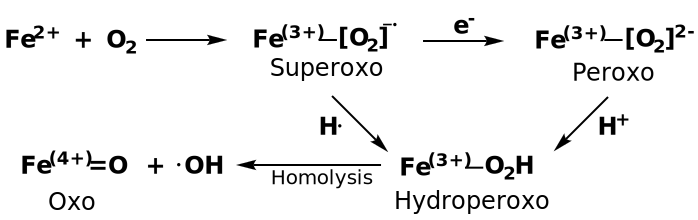
\includegraphics[width=0.8\textwidth]{Figures/Dioxygen_NHFe.pdf}
    \caption{General strategy for dioxygen activation by mononuclear non-heme iron enzymes. Adapted from \cite{Ray2014}.}
    \label{fig:NHFe_O2}
\end{figure}

The most common and best understood active species is iron(IV)-oxo. It has been trapped and characterized in synthetic biomimetic complexes \cite{Visser2013} in addition to being confirmed as the active species of many enzymes, e.g., tyrosine hydroxylase \cite{Eser2007} and taurine dioxygenase \cite{Gelasco2004}. The high-spin $S=2$ state is the ground state in mononuclear NHFe enzymes, whereas the $S=1$ state is found in heme iron(IV)-oxo species and synthetic complexes. A B3LYP cluster study suggests that the nature of the species performing HAA is best described as an iron(III)-oxyl radical \cite{Ye2011}. Theoretical studies show that HAA in the $S=1$ state proceeds only through a $\pi$ channel requiring perpendicular approach of the C-H bond to the iron(IV)-oxo bond \cite{Decker2007}. On the other hand, the $S=2$ state has both $\pi$ and $\sigma$ channels available.  

The iron(III)-superoxo species is suggested to perform HAA in the mononuclear NHFe enzyme IPNS \cite{Brown2007}, but a DFT study showed that it is in general less reactive than iron(IV)-oxo \cite{Chung2011}. No examples of HAA reactions performed by mononuclear iron(III)-peroxo species are known, while iron(III)-hydroperoxo is suggested as the active species in HAA from DNA by the anticancer drug bleomycin \cite{Chow2008}. An experimental study showed that both low- and high-spin synthetic iron(III)-hydroperoxo species are able to perform HAA \cite{Liu2013}.
 

\subsection{Dioxygen activation in binuclear NHFe enzymes}
The chemistry becomes more complex and challenging in the case of diiron sites. Binuclear NHFe enzymes can be further divided into two families: soluble and transmembrane enzymes. Significantly more is known about soluble enzymes, presumably because of the challenging nature of transmembrane proteins. X-ray diffraction experiments show that diiron sites in soluble enzymes contain a coordination environment rich in bridging carboxylate ligands with an iron-iron distance between 2.7 and 4.1 Å \cite{Jasniewski2018}. The resting state is in most cases an antiferromagnetically coupled high-spin Fe$^{\mathrm{II}}_{2}$ site. The presence of two iron centers, together with different coordination environments, results in diverse dioxygen activation mechanisms. Still, a common step for all of them is the step-wise reduction of dioxygen by electrons from iron ions. Figure \ref{fig:NHFe2_strategy} shows some of the most common reactive species and a general strategy for reaching them. We can see that they differ from species found in mononuclear enzymes in the fact that they are bridged iron-oxygen complexes.

\begin{figure}[htbp]
    \centering
    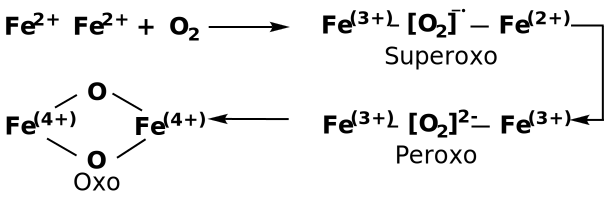
\includegraphics[width=0.7\textwidth]{Figures/Dioxygen_NHFe2.pdf}
    \caption{General strategy for dioxygen activation by soluble binucelar non-heme iron enzymes. Adapted from \cite{Ray2014}.}
    \label{fig:NHFe2_strategy}
\end{figure}

On the other hand, the diiron site in transmembrane enzymes is completely different. Strong evidence for this are the determined crystal structures of mouse and human stearoyl-CoA desaturase \cite{Bai2015,Wang2015}. One iron ion is coordinated by 5 histidine residues and the other with 4 histidines and one water molecule. The iron ions are separated by more than 6 Å, much larger than in soluble enzymes. This is possibly explained by the lack of carboxylate bridging ligands. Other representative members of this family are the alkane $\omega$-hydroxylase (AlkB) and xylene monooxygenase. Sequence comparisons showed that the coordinating histidines are conserved among all the members of the family \cite{Shanklin1994}. This can also be seen by comparing the predicted AlphaFold structures of AlkB and xylene monooxygenase with the crystal structure of SCD1 \cite{Varadi2022}. Furthermore, Chain et~al.~recently published a cryo-electron microscopy structure of AlkB from \textit{Fontimonas thermophila} fused with its electron donor protein \cite{Chai2023}. It shows the same nine histidine diiron site as in SCD1 but with a glutamate coordinated to one iron ion instead of a water molecule (Fig. \ref{fig:AlkB_structure}). The iron-iron distance is 6.1 Å. The large iron-iron distance in transmembrane enzymes possibly prohibits the formation of bridged iron-oxygen complexes and implies a completely different dioxygen activation mechanism compared to soluble enzymes. This claim must be tested because M\"ossbauer spectroscopy data on AlkB suggests the formation of bridged oxo complexes \cite{Shanklin1997}. This would require a reduction of the iron-iron distance by several Å~\cite{Shu1997}.

\begin{figure}[htbp]
    \centering
    \includegraphics[width=0.7\textwidth]{Figures/8f6t.png}
    \caption{Structure of the active site of alkane $\omega$-hydroxylase (AlkB) determined by cryo-electron microscopy with 2.76 Å resolution (PDB: 8F6T, \cite{Chai2023}). Residues are shown as sticks. Distance is shown in Å. Colours: pink, iron; red, oxygen; blue, nitrogen; white, carbon.}
    \label{fig:AlkB_structure}
\end{figure}


\section{Stearoyl-CoA desaturase}
Fatty acids are carboxylic acids with a 4 to 36 carbon long, usually linear, aliphatic chain \cite{Lehninger}. They are the main component of biological membranes and play an important role in energy storage and signalling. Based on the degree of saturation we divide them into: saturated, monounsaturated, and polyunsaturated fatty acids. Because of this, it is common to name unbranched fatty acids by only specifying the number of carbon atoms and the number of double bonds. The positions of the double bonds are indicated in the superscript of $\Delta$. Following this naming convention, stearic acid is named 18:0 because it is an 18 carbon saturated fatty acid. Similarly, oleic acid is 18:1($\Delta^{9}$) because it has one double bond after carbon 9 (counting from the carbonyl group). Fatty acids are rarely found as free carboxylic acids in biological systems, but rather in the form of esters and thioesters with various hydrophilic head groups.

SCD1 is an important enzyme in the fatty acid metabolism \cite{Paton2009}. It is a transmembrane protein of the endoplasmic reticulum (ER) and catalyzes the conversion of saturated to monounsaturated fatty acids (Fig.\,\ref{fig:SCD1_reaction}). The fatty acids need to be in the form of thioesters of coenzyme A (acyl-CoA). Desaturation is a two-electron oxidation, while the total reduction of O\textsubscript{2} requires four electrons. Two additional electrons are transported to SCD1 via an electron transport chain consisting of NAD(P)H, cytochrome b\textsubscript{5} reductase and cytochrome b\textsubscript{5}. The reaction is highly regio- and stereospecific. The introduced double bond is almost exclusively a \textit{cis}-9 double bond.

\begin{figure}[htbp]
    \centering
    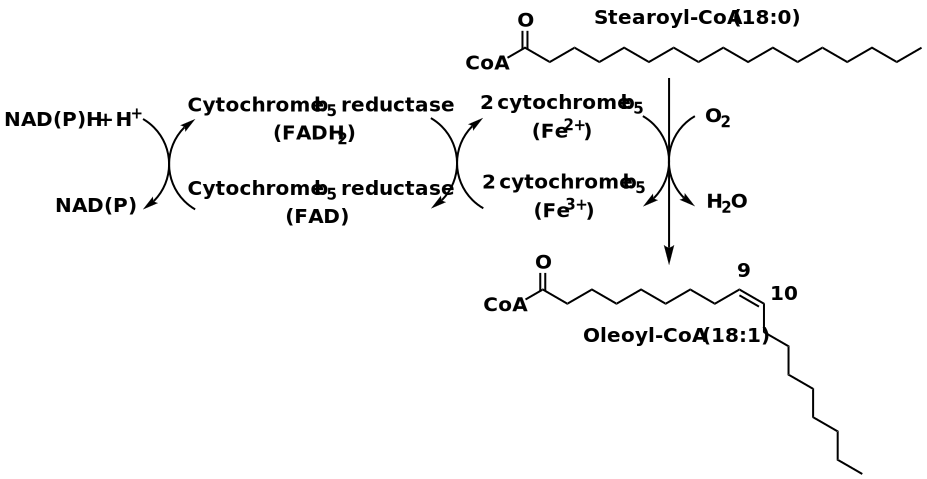
\includegraphics[width=\textwidth]{Figures/SCD1_reaction.pdf}
    \caption{Reaction catalyzed by stearoyl-CoA desaturase together with the electron transport chain. Adapted from \cite{Paton2009}.}
    \label{fig:SCD1_reaction}
\end{figure}

\subsection{Structure}
The function of SCD1 can be explained by looking at the determined crystal structures with stearoyl-CoA \cite{Bai2015,Wang2015}. It has a transmembrane and cytosolic domain (Fig.\,\ref{fig:SCD1_structure}). The transmembrane domain consists of 4 hydrophobic helices forming a wedge with the narrow side orientated towards the ER lumen. Conserved polar residues in the cytosolic domain interact with the hydrophilic CoA group and there is a H-bond between Trp258 and the acyl oxygen. A study on rat SCD1 found that free fatty acids cannot bind to the enzyme \cite{Enoch1976}, implying the importance of CoA for substrate binding. The aliphatic chain of stearoyl-CoA is placed inside a 24 Å long and narrow tunnel. The tunnel forms a turn near the dimetal active site (Fig.\,\ref{fig:SCD1_structure}). It is proposed that the turn is maintained with H-bonds between residues Trp149, Thr257 and Gln143. MD simulations on SCD1 support this claim \cite{Petroff2021}. These observations provide an explanation of the regio- and stereospecificity. Interactions with CoA and the acyl oxygen anchor the beginning of the chain while the turn of the tunnel forces the chain into a negative \textit{gauche} conformation suitable for \textit{cis}-9 double bond formation. 

The reported structures crystallized with Zn$^{2+}$ instead of Fe$^{2+}$ which is probably an artefact of overexpression \cite{Bai2015,Wang2015}. It is assumed that this does not affect the structure of the protein and the active site. This was confirmed by Shen et\,al.\,\cite{Shen2020} who managed to crystallize SCD1 with iron ions. No significant changes compared with the Zn structures were observed. In the structure of mouse SCD1 by Bai et\,al.\,\cite{Bai2015}, the metal ions are separated by 6.4 Å (Fig.\,\ref{fig:SCD1_structure}). One ion is coordinated by five histidines and the other by four histidines and one water molecule. C9 and C10 of stearoyl-CoA are close to the metal ions. Eight of the nine histidines are highly conserved in all transmembrane NHFe enzymes \cite{Shanklin1994}. The coordinated water molecule forms a hydrogen bond with the side chain amide nitrogen of Asn261, but based on the rest of the protein environment a bond with the amide oxygen would seem more favorable (Fig.\,\ref{fig:Crystal_water}). Determining the correct orientation of the Asn side chain is known to be problematic due to similar N/O electron densities \cite{Word1999}.

\begin{figure}[htbp]
    \centering
    \includegraphics[width=1.0\textwidth]{Figures/SCD1.png}
    \includegraphics[width=0.7\textwidth]{Figures/scd1_active_site.png}
    \caption{Structure of mouse stearoyl-CoA desaturase in complex with substrate (PDB: 4YMK, \cite{Bai2015}) with a schematic representation of membrane position (top) and geometry of the active site (bottom). Stearoyl-CoA and the active site are shown as sticks. Distances are shown in Å. Colours: silver, zinc; red, oxygen; blue, nitrogen; white, protein carbons; yellow, carbons of stearoyl-CoA and sulfur; orange, phosphorus.}
    \label{fig:SCD1_structure}
\end{figure}


\subsection{Substrate selectivity}
 Enoch et\,al.\,studied the activity of rat SCD1 with acyl-CoA substrates of varying chain lengths \cite{Enoch1976}. SCD1 was active for substrates with aliphatic chains containing between 12 and 19 carbons (Table\,\ref{tab:Enoch_table}). The highest activity is observed for substrates with 17 to 19 carbons. Interestingly, there is a very sharp drop off in activity for eicosanoyl-CoA (20:0). The determined crystal structures offer an explanation of the activity trends \cite{Bai2015}. The short acyl-CoA substrates are not able to reach the turn near the active site, whereas substrates with more than 19 carbons cannot fit into the tunnel. The residues Tyr104 and Ala108 at the end of the tunnel are suggested to limit the maximum chain length. Both residues are highly conserved in animal SCD1. A desaturase from \textit{Calanus hyperboreus} contains a smaller Thr residue in the position of the bulky Tyr104 which possibly explains its preference for long fatty acid substrates (22:0-26:0). Furthermore, mutagenesis studies showed that mutation of Thr to Tyr results in a loss of activity for long chain fatty acids \cite{Meesapyodsuk2014}. Another desaturase from \textit{Drosophilia melanogaster} has a larger Met residue in the position of Ala108 and is only active with fatty acids containing up to 14 carbon atoms \cite{Dallerac2000}.


\subsection{Reaction mechanism}
The desaturation reaction requires the abstraction of two hydrogen atoms, one from C9 and one from C10. This raises the question whether the two HAAs occur simultaneously or in two distinct steps. If the latter is the case, what is the site of initial abstraction? A comparative kinetic isotope effect (KIE) study on SCD1 suggests answers for these questions \cite{Buist1996}. In it, the reaction rate constants are compared for non-deuterated stearoyl-CoA ($k_H$) and for stearoyl-CoA deuterated at C9, and at C10 ($k_D$). The results show a large primary KIE for the C9 deuterated sample (${k_H}/{k_D}\simeq 5-8$) and a very small KIE for the C10 deuterated sample (${k_H}/{k_D}\simeq 1$). This rules out the simultaneous HAA mechanism and suggests initial slow rate-limiting HAA at C9 followed by fast HAA at C10. In support of this mechanism is a study which showed that SCD1 is more efficient at oxidizing the 9-thia analogue of stearoyl-CoA to sulfoxide than the 10-thia analogue \cite{Buist1992}.

SCD1 is a transmembrane binuclear NHFe enzyme and, as was discussed earlier, the identity of the iron-oxygen species responsible for desaturation is not known. Spectroscopic data on AlkB suggests formation of bridged iron-oxygen complexes \cite{Shanklin1997}, but it is not clear if that is possible based on the long iron-iron distance. A cluster model DFT/B3LYP study of the SCD1 active site investigated different possible desaturation mechanisms \cite{Yu2019}. All attempts at finding bridged iron-oxygen species resulted in oxygen binding to just one of the iron ions suggesting a novel oxygen activation mechanism. The full proposed reaction mechanism is shown in figure\,\ref{fig:SCD1_mechanism}. Oxygen binds to the tetracoordinated iron ion (Fe\textsubscript{B}) forming the typical iron(III)-superoxo species (React$_{\alpha}$) which gets transformed to iron(III)-hydroperoxo (Int1$_{\alpha}$, Int2$_{A-\alpha}$). Next, the O$-$O bond breaking is facilitated by hydrogen transfer from a water molecule activated by the other iron ion (Fe\textsubscript{A}) forming a triple-hydroxo intermediate (Int3$_{A-\alpha}$). This is suggested as the rate-limiting step in the proposed mechanism with a barrier of 13.4 kcal/mol. Proton transfer between the two hydroxides on Fe\textsubscript{B} leads to the formation of a high-valent iron(IV)-oxo species (Int4$_{A-\alpha}$) which can abstract the first hydrogen on C9 with a barrier of 10 kcal/mol (Fig.\,\ref{fig:Desaturation}). This is followed by a rapid second HAA from C10 by the hydroxide on Fe\textsubscript{A}. Transfer of an electron regenerates the initial state of the active site. The proposed mechanism is consistent with the KIE results which suggest that HAA on C9 is slow and occurs first. It also provides a nice explanation of the asymmetrical coordination of the iron ions. The tetracoordinated iron needs to have two free coordination positions to accommodate the two groups formed after O$-$O bond breaking while the other iron ion only needs one free position for water activation. Still, more experimental and computational data is necessary to validate the proposed mechanism and there is still the question of how to explain the AlkB spectroscopy data.  

\begin{figure}[htbp]
    \centering
    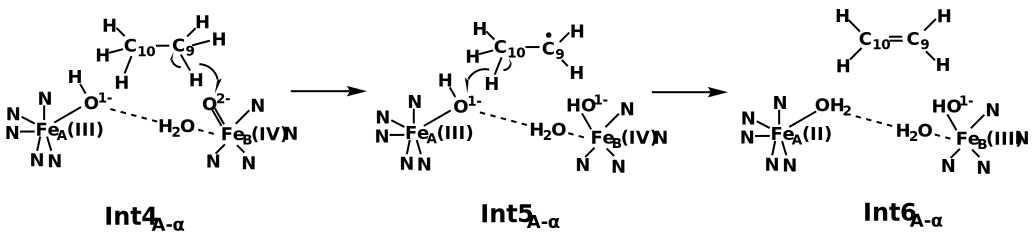
\includegraphics[width=\textwidth]{Figures/Desaturation_steps.pdf}
    \caption{Hydrogen atom abstraction steps in the proposed mechanism of stearoyl-CoA desaturase. Adapted from \cite{Yu2019}.}
    \label{fig:Desaturation}
\end{figure}

\subsection{SCD1 as a drug target}
Changes in fatty acid metabolism are linked with many diseases. As SCD1 is a key enzyme in fatty acid metabolism, it is a promising drug target. SCD1 inhibitors are studied for the potential treatment of obesity and type two diabetes \cite{Dobrzyn2005}. Studies showed that mice lacking the gene for SCD1 had increased sensitivity to insulin and were resistant to diet-induced obesity \cite{Ntambi2002}. It is suggested that SCD1 deficiency promotes partitioning of fats towards oxidation and in this way protects mice from obesity.

Normal tissue cells usually make use of circulating lipids. Cancer cells, on the other hand, have poor vascularization which results in a higher need for \textit{de novo} lipid synthesis \cite{Ackerman2014}. Membrane lipids are also required to facilitate the rapid growth of cancers \cite{Snaebjornsson2020}. Elevated lipid synthesis was connected to increased tumor growth \cite{Swinnen2006}. Expression of SCD1 was found to be elevated in several human cancer cell lines, including breast cancer \cite{Holder2013}, bladder cancer \cite{Presler2018} and kidney cancer \cite{Wang2015}. The studies also found correlation between higher concentrations of SCD1 and tumor malignancy as well as poorer chances of patient survival.

SCD1 inhibitors indeed show promising results in \textit{in vitro} studies but only few reached clinical testing due to strong side effects \cite{Zhang2014}. Besides the importance in cancer cells, SCD1 is essential for normal functioning of sebum-producing epithelial cells (sebocytes) \cite{Schneider2010}. Sebum is a waxy, oily mixture extracted on the skin, hair and eyes. It reduces evaporation and prevents heat loss. Although mice lacking SCD1 showed resistance to diet-induced obesity \cite{Ntambi2002}, lack of SCD1 also causes severely dry skin and eyes \cite{Miyazaki2001} in addition to hypothermia after exposure to cold \cite{Lee2004}. Tissue specific SCD1 inhibitors do posses better safety properties \cite{Zhang2014}.

Interesting progress in the field was made by Theodoropoulos et\,al.\,who managed to discover tumor-specific irreversible inhibitors of SCD1 \cite{Theodoropoulos2016}. The pro-drug is non-toxic for sebocytes and is selectively activated into an irreversible SCD1 inhibitor in cancer cells by cytochrome P450 (CYP) oxidases. CYPs metabolize drugs and other xenobiotics and are expressed in many cancer cells \cite{Rodriuez2006}. The pro-drug is activated by demethylation exposing a phenol group in the activated drug which irreversibly binds to SCD1, potentially in the diiron active site. The exact binding mechanism is not known but it is suggested to proceed through the formation of phenolic radical species \cite{Winterton2018}. CYPs are also expressed in the liver, but studies on mice showed that SCD1 is not essential in the liver \cite{Miyazaki2007}.


\section{Research goals}
The primary objective of this thesis is to further study the reactive intermediate of SCD1 proposed by Yu and Chen based on a B3LYP cluster model study (Int4$_{A-\alpha}$ from figure \ref{fig:Desaturation}) \cite{Yu2019}. Classical molecular dynamics simulations will be used to explore different conformations of the system. As a prerequisite it will be necessary to prepare the challenging membrane system and develop force field parameters for the metal center. The final goal is to study the intermediate's reactivity with QM/MM molecular dynamics simulations using the semiempirical GFN2-xTB QM method \cite{Bannwarth2019,Bannwarth2020,Grimme2017} combined with higher-level of theory energy corrections. GFN2-xTB showed very good performance in the prediction of the geometry of a diverse set of organometallic transition-metal complexes \cite{Bursch2019}, but to test its performance for the study of the HAA step by Int4$_{A-\alpha}$ a cluster model potential energy surface (PES) scan will be performed and results compared to the reported B3LYP results.

The study will provide a better understanding of the selectivity and reactivity of SCD1 which can help in the design of new inhibitors but also provide insight into the poorly understood mechanism of the whole group of transmembrane NHFe$_2$ enzymes. To the best of our knowledge this will be the first application of multiscale molecular dynamics simulations for the study of reactivity of a transmembrane NHFe$_2$ enzyme. 


\chapter{Theory}

\section{A brief introduction to statistical mechanics}
The discussion in this section is mostly based on the ``Introduction to Computational Chemistry'' textbook written by Jensen~\citep{jensenIntroductionComputationalChemistry2017}, ``Statistical Mechanics: Theory and Molecular Simulation'' by Tuckermann~\citep{tuckermanStatisticalMechanicsTheory2023}, and ``Understanding Molecular Simulation: From Algorithms to Applications'' by Frenkel and Smit~\citep{frenkelUnderstandingMolecularSimulation2002} unless stated otherwise.



\subsection{Partition functions}
The development of the field of statistical mechanics has been crucial for the computational chemistry community, as it enables the connection between the jigglings and wigglings of atoms and the properties of much larger systems such as liquids and solids.

Let us begin with the most fundamental concept: the partition function. The partition function is akin to a Swiss army knife in statistical mechanics, meaning it is a versatile tool that makes the connection between microscopic and macroscopic properties in thermodynamics possible. In the simplest case of a single molecule, the partition function $q$ takes the following form:

\begin{equation}
    q = \sum_{i = \text{levels}}^{\infty} g_i e^{-\epsilon_i/kT}
\end{equation}

Here, it is expressed as a sum over all energy levels $\epsilon_i$ of a molecule (or particle), multiplied by a degeneracy factor $g_i$ in cases where multiple levels have the same energy. The term $kT$ represents the Boltzmann factor.

Moving on to a more complex scenario in which the partition function describes multiple molecules, we arrive at the partition function $Q$ for non-interacting particles, such as those in an ideal gas:

\begin{equation}
    \label{eq:Q_noninteracting}
    Q = q^N \; \text{(different particles)} \quad Q = \frac{q^N}{N!} \; \text{(identical particles)}
\end{equation}

Here, $N$ denotes the total number of particles. However, one could argue that if we wish to describe a real system such as bulk water, we must account for interactions between molecules. Consequently, Equation~\ref{eq:Q_noninteracting} must be rewritten:

\begin{equation}
    Q = \sum_{i}^{\infty} e^{-E_i/kT}
\end{equation}

In this case, the partition function $Q$ includes contributions from all possible energy states $E_i$ of the system.

Although the concept of the partition function might initially appear abstract, it can be clarified by expressing it in a different form, namely, within the context of the \ac{rrho} approximation, where the electronic, vibrational, and rotational degrees of freedom can be separated. For a single molecule case it would look like:

\begin{equation}
    q_{\text{tot}} = q_{\text{trans}} \times q_{\text{rot}} \times q_{\text{vib}} \times q_{\text{elec}}
\end{equation}

Let us now examine each contribution in more detail. From this point onward we will consider polyatomic molecules in the formulation of the partition functions, unless stated otherwise.

The translational partition function $q_\text{trans}$ can be derived from the energy expression for a particle in a one-dimensional box and is given by:

\begin{equation}
    q_{\text{trans}} = \left(\frac{2\pi MkT}{h^2}\right)^{3/2} V
\end{equation}

Here, $M$ is the total molecular mass, and $V$ is the volume. Turning to the rotational partition function $q_\text{rot}$, it can be derived from the Schr\"odinger equation for a diatomic "rigid rotor" and has the following form:

\begin{equation}
    q_{\text{rot}} = \frac{8\pi^2IkT}{h^2\sigma}
\end{equation}

In this expression, $I$ denotes the moment of inertia, and $\sigma$ represents the symmetry factor, i.e. the order of the rotational subgroup within the molecular point group. For polyatomic molecules, writing an exact expression is more complex, but an approximate form can be used:

\begin{equation}
    q_{\text{rot}} = \frac{\sqrt{\pi}}{\sigma}\left(\frac{8\pi^2kT}{h^2}\right)^{3/2} \sqrt{I_1I_2I_3}
\end{equation}

For the vibrational partition function $q_\text{vib}$, it is expressed as a product over the various vibrational modes of a molecule, each with frequency $\nu_i$:

\begin{equation}
    q_{\text{vib}} = \prod_{i} \frac{e^{-h\nu_i/2kT}}{1-e^{-h\nu_i/kT}}
\end{equation}

Lastly, the electronic partition function $q_\text{elec}$ is given as a sum over all electronic states of a molecule, from the ground state to all excited states. However, since the energy difference between the ground state and higher states is usually much greater than $kT$ at ambient temperatures, the function can typically be approximated by considering only the ground state:

\begin{equation}
    q_{\text{elec}} = \sum_{i=0}^{\infty} g_i e^{-\epsilon_i/kT} \approx g_0 e^{-\epsilon_0/kT}
\end{equation} 



\subsection{Macroscopic properties and thermodynamic functions}

Once the partition function is determined, it provides a direct means of evaluating macroscopic properties. For instance, the internal energy $U$ and the Helmholtz free energy $A$ can be calculated from the partition function $Q$:

\begin{align}
    U &= kT^2 \left(\frac{\partial \ln Q}{\partial T}\right)_V \\
    A &= -kT\ln Q
\end{align}

In addition, other macroscopic properties, such as pressure $P$ and the heat capacity at constant volume $C_V$, can also be expressed in terms of the partition function:

\begin{align}
    P &= -\left(\frac{\partial A}{\partial V}\right)_T = kT\left(\frac{\partial \ln Q}{\partial V}\right)_T \\
    C_V &= \left(\frac{\partial U}{\partial T}\right)_V = 2kT\left(\frac{\partial \ln Q}{\partial T}\right)_V + kT^2\left(\frac{\partial^2 \ln Q}{\partial T^2}\right)_V
\end{align}

Turning to thermodynamic functions, namely enthalpy $H$, entropy $S$, and Gibbs free energy $G$, these can also be derived from the partition function $Q$:

\begin{align}
    H &= U + PV = kT^2\left(\frac{\partial \ln Q}{\partial T}\right)_V + kTV\left(\frac{\partial \ln Q}{\partial V}\right)_T \\
    S &= \frac{U-A}{T} = kT\left(\frac{\partial \ln Q}{\partial T}\right)_V + k\ln Q \\
    G &= H - TS = kTV\left(\frac{\partial \ln Q}{\partial V}\right)_T - kT\ln Q
\end{align}

This connection between macroscopic observables, thermodynamic functions, and the partition function once again highlights its fundamental importance in statistical thermodynamics.



\subsection{The canonical ensemble}
Having established a method to calculate the macroscopic properties of a system we implicitly relied on averaging over a large enough number of states. Therefore one may naturally ask: how can we sample enough configurations to apply the equations described in the previous section under conditions that resemble those in experiments? One such answer is the canonical ensemble.

The canonical ensemble describes a system at constant temperature $T$, fixed volume $V$, and a fixed number of particles $N$ (\acs{nvt}). In this ensemble, the system is in contact with a heat bath, which makes it particularly relevant to most molecular simulations that are describing the experimental conditions, where the temperature is externally controlled while the internal energy of the system is allowed to fluctuate.

Since the energy fluctuates in the canonical ensemble, a logical step is to estimate the magnitude of these fluctuations:

\begin{equation}
    \frac{\Delta E}{E} \sim \frac{\sqrt{N}}{N} \sim \frac{1}{\sqrt{N}}
\end{equation}

Here, $N$ denotes the number of particles, and thus for sufficiently large systems, the relative energy fluctuations become negligible.

The use of the canonical ensemble implicitly assumes that the system is ergodic, meaning that time averages obtained from simulation trajectories are equivalent to ensemble averages over the Boltzmann distribution. This assumption is, for instance, central to molecular dynamics simulations where the canonical ensemble can be sampled.



\subsection{Classical forcefields and molecular dynamics}
Bringing all the puzzle pieces together, we can now discuss how to simulate a molecular or atomic system of interest. One widely used approach is \ac{md} simulations. The first step involves defining a potential energy function that describes the interactions between atoms. This function, often referred to as a forcefield, is typically parameterised based on experimental data or high-level quantum mechanical calculations.

In classical \ac{md}, the evolution of a system of $N$ atoms is governed by Newton's equations of motion. A commonly used form of the potential energy function is:

\begin{equation}
\begin{aligned}
    U(\mathbf{r}_1, \dots, \mathbf{r}_N) = &\sum_{\text{bonds}} \frac{1}{2} K_{\text{bond}} (r - r_0)^2 + 
    \sum_{\text{bends}} \frac{1}{2} K_{\text{bend}} (\theta - \theta_0)^2 \\
    &+ \sum_{\text{tors}} \sum_{n=0}^{6} A_n \left[ 1 + \cos(C_n \phi + \delta_n) \right] \\
    &+ \sum_{i,j \in \text{nb}} \left\{ \left[ 4\epsilon_{ij} \left( \frac{\sigma_{ij}}{r_{ij}} \right)^{12}
    - \left( \frac{\sigma_{ij}}{r_{ij}} \right)^6 \right] + \frac{q_i q_j}{r_{ij}} \right\}
\end{aligned}
\label{eq:md_potential}
\end{equation}

Here, the total energy is decomposed into bonded interactions (bonds, angles, and torsions) and non-bonded interactions, including Lennard-Jones and Coulombic terms. Once the potential is specified, the force on each atom $i$ is obtained via:

\begin{equation}
    \mathbf{F}_i = -\frac{\partial U}{\partial \mathbf{r}_i}
    \label{eq:md_force}
\end{equation}

To propagate the positions and velocities of atoms in time, numerical integration schemes are employed. Among these, the velocity Verlet algorithm is widely used in perhaps all \ac{md} engines. Let us consider the Taylor expansion of the position of particle $i$ to second order in the time step $\Delta t$:

\begin{equation}
    \mathbf{r}_i(t + \Delta t) \approx \mathbf{r}_i(t) + \Delta t\, \mathbf{v}_i(t) + \frac{\Delta t^2}{2m_i} \mathbf{F}_i(t)
    \label{eq:vv_pos}
\end{equation}

Here, $\mathbf{F}_i(t)$ is the force on particle $i$ at time $t$, and $m_i$ is its mass, calculated using Equation~\ref{eq:md_force} and $\mathbf{v}_i(t)$ is its velocity. This expression provides a prediction of the new position based on the current velocity and force.

We can also consider a backward expansion in time from $\mathbf{r}_i(t + \Delta t)$ and $\mathbf{v}_i(t + \Delta t)$, yielding:

\begin{equation}
    \mathbf{r}_i(t) = \mathbf{r}_i(t + \Delta t) - \Delta t\, \mathbf{v}_i(t + \Delta t) + \frac{\Delta t^2}{2m_i} \mathbf{F}_i(t + \Delta t)
    \label{eq:vv_pos_backward}
\end{equation}

By substituting Equation~\ref{eq:vv_pos} into Equation~\ref{eq:vv_pos_backward} and solving for $\mathbf{v}_i(t + \Delta t)$, we get:

\begin{equation}
    \mathbf{v}_i(t + \Delta t) = \mathbf{v}_i(t) + \frac{\Delta t}{2m_i} \left[ \mathbf{F}_i(t) + \mathbf{F}_i(t + \Delta t) \right]
    \label{eq:vv_vel}
\end{equation}

Equations~\ref{eq:vv_pos} and \ref{eq:vv_vel} together form the velocity Verlet integrator. The algorithm proceeds as follows:
\begin{enumerate}
  \item First, update positions using Equation~\ref{eq:vv_pos}.
  \item Then, compute new forces $\mathbf{F}_i(t + \Delta t)$ based on the updated positions.
  \item Finally, update velocities using Equation~\ref{eq:vv_vel}.
\end{enumerate}

To correctly sample the canonical ensemble, one should consider the use of thermostats to maintain the system temperature. In this work, we focus on two widely used thermostats: the Nos\'e--Hoover thermostat~\citep{noseUnifiedFormulationConstant1984, hooverCanonicalDynamicsEquilibrium1985} and the \ac{csvr} thermostat~\citep{bussiCanonicalSamplingVelocity2007}. In the former, the equations of motion are modified to include a friction term that couples the system to a heat bath, allowing for energy exchange. The \ac{csvr} thermostat, on the other hand, uses a velocity rescaling approach to maintain the desired temperature by adjusting particle velocities at each time step.



\subsection{Enhanced sampling techniques}
Even though \ac{md} simulations are a powerful tool for studying molecular systems, their applicability can be limited due to the presence of energy barriers separating minima in the potential energy landscape. As a result, the system may remain trapped in local minima, leading to insufficient sampling of the relevant configurational space. This issue becomes particularly pronounced in the context of reactive systems, where rare events involve transitions between states separated by high free energy barriers and occur on timescales much longer than typical simulation durations.

To address this challenge, various enhanced sampling techniques have been developed. These methods aim to accelerate the exploration of phase space. In general, they bias the system along reaction coordinates, or \acp{cv}, by applying a biasing potential that drives the system towards regions of interest. One such approach is metadynamics~\citep{laioEscapingFreeenergyMinima2002, laioMetadynamicsMethodSimulate2008}.

In metadynamics, a biasing (external) potential is added to the system's potential energy surface. This biasing potential takes the following form:

\begin{equation}
    V_{\text{G}}(S(x), t) = w \sum_{t' = \tau_{\text{G}}, 2\tau_{\text{G}}, \ldots}^{t' < t} \exp\left(-\frac{(S(x) - s(t'))^2}{2\delta s^2}\right)
    \label{eq:biasing_potential}
\end{equation}

where $s(t) = S(x(t))$ is the value of the \ac{cv} at time $t$. The height of the Gaussian kernel is denoted by $w$, $\delta s$ is its width, and $\tau_{\text{G}}$ is the deposition rate.

The approach used in metadynamics can be explained using the Panama Canal as an analogy as illustrated in Figure~\ref{fig:metadynamics}. The idea is to fill the basins of the free energy landscape with a Gaussian potential, which can be thought of as water gradually filling the basins, lifting the system (like a ship in a lock) out of a free energy minimum and helping it traverse to other states.

The assumption in metadynamics is that, after sufficiently long sampling, the biasing potential $V_{\text{G}}(S, t)$ converges to the negative of the underlying free energy surface:

\begin{equation}
    \label{eq:free_energy_from_metadynamics}
    \lim_{t \to \infty} V_G(s,t) \sim -F(s)
\end{equation}

Despite the many benefits that metadynamics offers, it is important to note that it has limitations. For example, obtaining a converged free energy surface is not straightforward, especially when multiple \acp{cv} are involved. In principle, Gaussian kernels can be deposited indefinitely, making it difficult to assess convergence. To address this issue, the well-tempered variant of metadynamics was developed~\citep{barducciWellTemperedMetadynamicsSmoothly2008}. In this method, a history-dependent potential is added, which is defined as:

\begin{equation}
    V(s, t) = \Delta T \ln\left(1 + \frac{\omega N(s, t)}{\Delta T}\right)
    \label{eq:history_dependant_potential}
\end{equation}

Here, $N(s, t)$ is the histogram of $s$ obtained from a biased simulation, $\Delta T$ is the biasing temperature, and $\omega$ has the dimension of an energy rate. The rate at which this potential is modified over time is given by:

\begin{figure}[b!]
    \centering
    \includegraphics[width=0.8\textwidth]{Figures/2_Theory/theory_metadynamics.png}
    \caption{The concept of metadynamics. $w$ stands for the Gaussian kernel height, and $\delta s$ stands for its width. The Panama Canal cartoon was reproduced from~\citep{HowPanamaCanal}.}
    \label{fig:metadynamics}
\end{figure}

\begin{equation}
    \dot{V}(s,t) = \frac{\omega \Delta T \delta_{s,s(t)}}{\Delta T + \omega N(s,t)} 
    = \omega e^{-[V(s,t)/\Delta T]} \delta_{s,s(t)}
    \label{eq:hill_deposition_rate}
\end{equation}

The height of the Gaussian kernels used is:

\begin{equation}
    w = \omega e^{-[V(s,t)/\Delta T]} \tau_{\text{G}}
    \label{eq:hill_height}
\end{equation}

where $\tau_{\text{G}}$ is the deposition rate and $\omega$ represents the initial bias deposition rate. The Gaussian kernel height is now dependent on the history of the system, allowing for a more controlled exploration of the free energy landscape.

Ultimately, the underlying free energy surface can be estimated using the following equation:

\begin{equation}
    \tilde{F}(s,t) = -\frac{T + \Delta T}{\Delta T} V(s,t) 
    = -(T + \Delta T) \ln\left(1 + \frac{\omega N(s,t)}{\Delta T} \right)
    \label{eq:free_energy_surface_reconstruction}
\end{equation}

The advantage of \ac{wtmd} is that it enables more efficient exploration of the free energy landscape, as the biasing potential adapts according to the trajectory's history. Moreover, the convergence can be easily monitored by observing the decay of the Gaussian height, which should approach zero as the system fully explores the relevant phase space.



%%%%%%%%%%%%%%%%%%%%%%%%%%%%%%%%%%%%%%%%%%%%%%%%%%%%%%%%%%%%%%%%%%%%%%%%%%%%%%%%

% \section{Transition state theory}



%%%%%%%%%%%%%%%%%%%%%%%%%%%%%%%%%%%%%%%%%%%%%%%%%%%%%%%%%%%%%%%%%%%%%%%%%%%%%%%%

\section{The density functional theory tourist}
The discussion in this section is primarily based on the ``Introduction to Computational Chemistry'' textbook written by Jensen~\citep{jensenIntroductionComputationalChemistry2017}, ``Density Functional Theory: a Practical Introduction'' by Scholl and Steckel~\citep{shollDensityFunctionalTheory2011}, and ``A Chemist's Guide to Density Functional Theory'' by Koch and Holthausen~\citep{kochChemistsGuideDensity2015} unless stated otherwise.

\subsection{The Kohn-Sham approach}
In order to describe reactive events in relatively large systems, up to approximately 1,000 atoms, it is necessary to use methods that offer a good balance between accuracy and computational cost. One such method is \ac{dft}, which is based on the Hohenberg-Kohn theorems and the Kohn-Sham equations.

The central idea behind \ac{dft}, established by Hohenberg and Kohn, is that the ground state energy of a many-electron system can be expressed as a functional of the electron density. This reformulation reduces the problem from solving a 3$N$-dimensional wavefunction to working with a 3-dimensional electron density.

The energy functional can be written as:

\begin{equation}
    \begin{aligned}
    E[\rho(\mathbf{r})] &= T_{\text{s}}[\rho] + J[\rho] + E_{\text{Ne}}[\rho] + E_{\text{XC}}[\rho] =  \\
    &= -\frac{1}{2} \sum_{i}^{N} \langle \phi_i | \nabla^2 | \phi_i \rangle \\
    &\quad + \frac{1}{2} \sum_{i}^{N} \sum_{j}^{N} \iint \left| \phi_i(\mathbf{r}_1) \right|^2 \frac{1}{r_{12}} \left| \phi_j(\mathbf{r}_2) \right|^2 d\mathbf{r}_1 d\mathbf{r}_2 \\
    &\quad - \sum_{i}^{N} \sum_{A}^{M} \int \frac{Z_A}{r_{1A}} \left| \phi_i(\mathbf{r}_1) \right|^2 d\mathbf{r}_1 \\
    &\quad + E_{\text{XC}}[\rho(\mathbf{r})] 
    \label{eq:ks_energy}
    \end{aligned}
\end{equation}

Here, the first three terms are “known” and represent the kinetic energy of the electrons, the Coulomb interaction between the electrons, and the electron-nucleus interaction, respectively. The final term, the exchange-correlation energy functional, is the unknown component. It contains all the effects that are not straightforward to treat exactly, for instance, the residual part of the kinetic energy and the non-classical electron-electron interactions:

\begin{equation}
    E_{\text{XC}}[\rho] \equiv (T[\rho] - T_{\text{s}}[\rho]) + (E_{\text{ee}}[\rho] - J[\rho])
    \label{eq:xc_energy}
\end{equation}

The biggest challenge in \ac{dft} lies in the formulation of $E_{\text{XC}}$. This term is particularly important, as finding the minimum of the total energy functional, as expressed in Equation~\ref{eq:ks_energy}, depends on its accurate representation.

To address this, the Kohn-Sham approach introduces a set of single-electron equations that can be solved iteratively to obtain the electron density and the total energy of the system. The Kohn-Sham equations are given by:

\begin{equation}
    \left( -\frac{1}{2} \nabla^2 + V_{\text{eff}}(\mathbf{r}) \right) \phi_i = \varepsilon_i \phi_i
    \label{eq:ks_equations}
\end{equation}

Here, $V_{\text{eff}}$ takes the form:

\begin{equation}
    V_{\text{eff}}(\mathbf{r}) = \int \frac{\rho(\mathbf{r}_2)}{r_{12}} d\mathbf{r}_2 + V_{\text{XC}}(\mathbf{r}) - \sum_{A}^{M} \frac{Z_A}{r_{1A}}
    \label{eq:v_eff}
\end{equation}

The iterative procedure to solve these equations proceeds as follows: first, a trial electron density is defined. Then, the Kohn-Sham equations are solved using this trial density to obtain the single-particle wavefunctions. Next, a new electron density is calculated from the obtained wavefunctions. Finally, the new density is compared with the initial trial density. If the two densities match within a given convergence criterion, the ground state electron density has been found, and the total energy of the system can be computed.



\subsection{Generalised gradient approximation and PBE functional}
The field of \ac{dft} has opened new avenues for computational chemists and physicists, enabling them to study the properties of materials and molecules, as well as to investigate the reaction pathways of chemical processes. However, the accuracy of \ac{dft} calculations is highly dependent on the choice of the exchange-correlation functional.

In this work, we focus on the \ac{gga} exchange-correlation functionals, which are widely used in \ac{dft} calculations and are known to provide results close to chemical accuracy at a relatively low computational cost, as can be seen in Figure~\ref{fig:jacobs_ladder}. In fact, the development of \ac{gga} functionals marked a turning point in the acceptance of the \ac{dft} method by the quantum chemistry community.

The \ac{gga} functionals are based on the idea that the exchange-correlation energy can be expressed as a functional of the electron density $\rho$ and its gradient $\nabla \rho$. The general form of a \ac{gga} functional is given by:

\begin{equation}
E_{\text{XC}}^{\text{GGA}}[\rho] = \int f(\rho, \nabla\rho) \, d\mathbf{r}
\label{eq:gga_functional}
\end{equation}

The exchange-correlation energy can be explicitly divided into two parts:

\begin{equation}
E_{\text{XC}}^{\text{GGA}} = E_{\text{X}}^{\text{GGA}} + E_{\text{C}}^{\text{GGA}}
\label{eq:gga_xc}
\end{equation}

One of the most widely used \ac{gga} functionals is the Perdew-Burke-Ernzerhof (PBE) functional~\citep{perdewGeneralizedGradientApproximation1996}. Its formulation incorporates parameters in the exchange and correlation parts derived from first principles, making it a truly \textit{ab initio} functional.

\begin{figure}[b!]
    \centering
    \includegraphics[width=0.7\textwidth]{Figures/2_Theory/theory_jacobs_ladder.png}
    \caption{Left panel: accuracy of the common quantum chemical methods as a function of the computatinal cost. Right panel: categorisation of the exchange-correlation functionals according to Perdew's ``Jacob's ladder''. The figure was reproduced from \citep{burschBestPracticeDFTProtocols2022}.}
    \label{fig:jacobs_ladder}
\end{figure}



\subsection{\textit{Ab initio} molecular dynamics}
In one of the previous sections, we touched upon the topic of classical \ac{md} simulations. However, classical force fields are unable to simulate bond-breaking and bond-forming processes. Although reactive events can also be studied using static approaches, by calculating the potential energy surface at a given set of coordinates, we believe that incorporating dynamics provides more informative insights and a clearer picture of the reaction mechanism.

To simulate the dynamics of a chemical reaction, one could consider using \ac{aimd}, and in particular, \ac{bomd}. In \ac{bomd}, the forces acting on the atoms are calculated at each time step using quantum mechanical methods, such as \ac{dft}, while the nuclei are propagated according to classical mechanics. This process can be described using the Lagrangian formalism, $L$, which offers an alternative formulation of classical dynamics:

\begin{equation}
L = K - U = \frac{1}{2} \sum_{i=1}^{3N} m_i v_i^2 - E[\phi(\mathbf{r}_1, \ldots, \mathbf{r}_{3N})]
\label{eq:lagrangian_aimd}
\end{equation}

where $K$ is the kinetic energy, $U$ represents the potential energy, and $\phi(\mathbf{r}_1, \ldots, \mathbf{r}_{3N})$ is a set of one-electron Kohn-Sham wave functions.

It is important to note that, since nuclear dynamics are treated classically in this framework, zero-point vibrational energy is not accounted for, nor can tunnelling effects be studied. 



%%%%%%%%%%%%%%%%%%%%%%%%%%%%%%%%%%%%%%%%%%%%%%%%%%%%%%%%%%%%%%%%%%%%%%%%%%%%%%%%

\section{Extended tight binding}



%%%%%%%%%%%%%%%%%%%%%%%%%%%%%%%%%%%%%%%%%%%%%%%%%%%%%%%%%%%%%%%%%%%%%%%%%%%%%%%%

\section{Neural network potentials}

\subsection{Message passing graph neural networks}

\subsection{Invariance and equivariance}

\subsection{Equivariant neural network potentials}
\chapter{Computational Details}
This chapter gives the computational details of all methods used in the thesis. The first section describes the system preparation and setup of classical molecular dynamics simulations. The MD simulations of the proposed reactive intermediate Int4$_{\text{A}-\alpha}$ suggest that it has unfavorable dynamical properties, so simulations of a newly proposed intermediate were also performed. From now on Int4$_{\text{A}-\alpha}$ is referred to as intermediate A while our newly proposed intermediate is referred to as intermediate B (Fig.\,\ref{fig:IntA_IntB}). They differ in the position of the oxo group on Fe$_{\text{B}}$. The second section gives details on the cluster model relaxed potential energy surface (PES) scan with GFN2-xTB \cite{Bannwarth2019,Grimme2017} for the HAA step by A which was used to assess the applicability of the GFN2-xTB method. The last section describes how QM/MM PES scans and MD simulations were used to study the reactivity of the newly proposed intermediate B.
\begin{figure}[htbp]
    \centering
    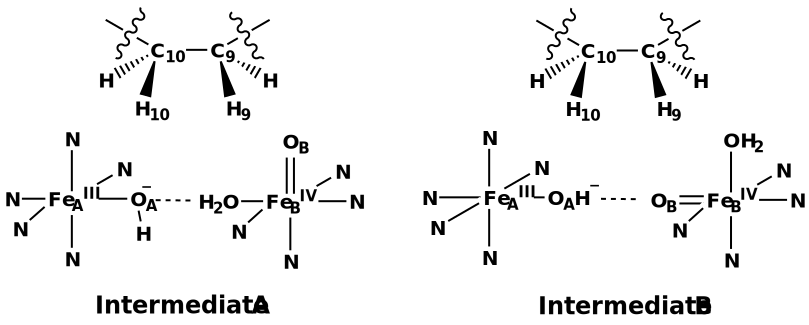
\includegraphics[width=0.8 \textwidth]{Figures/int_A_B.pdf}
    \caption{Schematic representation of the proposed reactive intermediate of SCD1 Int4$_{\text{A}-\alpha}$ by Yu and Chen (A) \cite{Yu2019} and our newly proposed intermediate B.}
    \label{fig:IntA_IntB}
\end{figure}

\section{Classical MD simulations}
\subsection{System preparation}
The membrane system was built from the crystal structure of mouse SCD1 (PDB: 4YMK \cite{Bai2015}) taken from the OPM database \cite{Lomize2012}. Missing residues at the N- and C-terminus were ignored. The cocrystallized [(Z)-octadec-9-enyl] (2R)-2,3-dihydroxypro\-pa\-noate was removed and zinc ions were replaced with iron. All crystal waters were removed except the ones around the active site and the substrate tunnel which were in a favourable protein environment. Hydrogens to stearoyl-CoA (ST9) were added using the reduce program from the AmberTools22 package \cite{ambertools22}. The protein's most probable protonation state at pH 7.4 was determined using the H++ web-server (version 4.0) \cite{H++,Myers2006,Gordon2005,Anandakrishnan2012}. It was necessary to manually correct the protonation state of two His residues around the iron ions to ensure correct coordination. The membrane consisting of 1-palmitoyl-2-oleoyl-sn-glycero-3-phosphocholine (POPC) around the protein was generated using the CHARMM-GUI membrane builder \cite{Jo2008}. The system was placed in a cubic box and solvated with water and 0.15 M NaCl (until neutral) where the distance of the protein to an edge of the box is at least 10 Å. The structure of the active site was manually modified to match the structures of intermediates A and B by adding the necessary ligands. 

\subsection{FF parameters}
The following public FFs were used to describe the system: ff19SB \cite{Tian2020} for protein residues; Lipid21 for membrane lipids; OPC \cite{Xiong2020} for water; Li and Merz 12-6 ions FF \cite{Sengupta2021} for the Na\textsuperscript{+} and Cl\textsuperscript{-} ions. 

ST9 was divided in three fragments (Fig.\,\ref{fig:ST9}). Bonded parameters and partial charges of the first fragment were taken from the parameters of the stearoyl acyl chain in the Lipid21 FF. Fragments 2 and 3, as well as interactions between 1 and 2, were described with GAFF2 \cite{He2020}. Partial charges of 2 and 3 were determined separately using the RESP method \cite{Bayly1993} with the py\_resp.py program from the AmberTools22 package. The ESP was calculated on the HF/6-31G* level of theory using Gaussian16 \cite{gaussian16}. Appropriate cap groups were placed at bond breaking points (methyl and acetyl for fragment 2, methylamine for fragment 3) and their charge restrained during RESP fitting to maintain the correct total molecular charge. The geometry of the fragments was optimized with GFN2-xTB prior to RESP fitting.
\begin{figure}[htbp]
    \centering
    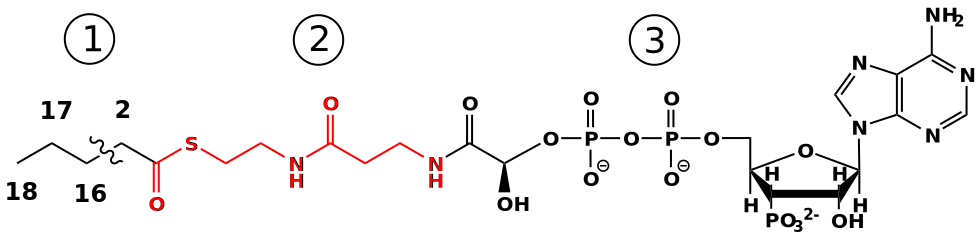
\includegraphics[width=1.0 \textwidth]{Figures/ST9.pdf}
    \caption{Splitting of stearoyl-CoA in three fragments for parameter determination.}
    \label{fig:ST9}
\end{figure}

Parameters for the diiron center of both intermediate A and B were determined with the help of the MCPB.py \cite{Li2016} program from the AmberTools22 package. Each iron ion was treated individually because there are no direct covalent bonds between the two centers. For each ion a small and a large model was generated. The smaller model was used for geometry optimization and the calculation of the Cartesian Hessian matrix with Gaussian16 on the B3LYP/6-31G* level of theory. Bond and angle parameters were determined from the Cartessian Hessian matrix using the Seminario method \cite{seminario1996}. This also includes the O$-$H bond and H$-$O$-$H angle parameters of the active site water ligand. All dihedral parameters were set to 0. The larger model was used for RESP partial charge fitting. The positions of hydrogens were optimized with GFN2-xTB prior to calculating the ESP with Gaussian16 on the B3LYP/6-31G* level of theory. In all calculations the high-spin states of the iron ions were assumed: $S=2$ for Fe(IV), $S=2.5$ for Fe(III). In the end it was necessary to treat the water molecule in the active site in a non-bonded way with harmonic restraints on the O$_\text{W}-$Fe$_\text{B}$ distance and O$_\text{W}-$Fe$_\text{B}-$O$_\text{B}$ angle. The force constant of restraint and the equilibrium value were set to match the parameters determined with the Seminario method. This was necessary because O$_\text{B}$ and water hydrogens show electrostatic attraction but there isn't any repulsion preventing their complete overlap when water is treated in a bonded way (the LJ parameters of hydrogens are zero and there isn't any electrostatic repulsion between O$_\text{W}$ and O$_\text{B}$ because they are only separated by two bonds). When water is treated in a non-bonded way there is electrostatic repulsion between O$_\text{W}$ and O$_\text{B}$ preventing nonphysical overlap of O$_\text{B}$ and water hydrogens. This is a known problem of bonded metal site models \cite{Li2017}.

\subsection{Equilibration and production}
The same equilibration protocol was used for both intermediates A and B. A more detailed overview of the equilibration procedure is shown in table \ref{tab:eq_protocol}. PBCs are used with the particle mesh Ewald method for computing electrostatic interactions \cite{Petersen1995} and a 10 Å cutoff for short-range interactions. First, a series of minimization runs was performed gradually releasing the constraints on the protein and membrane. This was followed by heating the system under constant volume from 0 to 100 K during a 5 ps simulation on a CPU with a constraint of 5 kcal mol$^{-1}$ Å$^{-2}$ on the positions of the protein, ST9 and the membrane. The heating until 300 K was continued on a GPU during 100 ps and constant pressure conditions (1 bar). Finally, the system was equilibrated under constant pressure conditions (1 bar) at 300 K in a series of equilibration runs. Constant temperature was maintained with a Langevine thermostat, while pressure was regulated with a semi-isotropic Berendsen barostat (box vectors in the membrane plane are coupled while the perpendicular vector was allowed to change freely). Three evenly spaced structures from the last 5 ns equilibration were taken as starting points for the three independent production runs (random velocity assignment) of 500 ns for intermediate A and 1 $\mu$s for intermediate B. Production was performed under 1 bar and 300 K on a GPU using a 2 fs timestep with the SHAKE algorithm \cite{Tobias1988} for constraining bonds with hydrogens. All GPU runs were performed with the Amber20 version of pmemd \cite{pmemd1,pmemd2} on one GPU, while all CPU runs were performed with sander.MPI using 8 MPI task. 

\subsection{Analysis}
Trajectories were visualized with visual molecular dyanmics \cite{HUMP96,STON1998}. Analysis was performed with cpptraj and pytraj from the AmberTools22 package \cite{Roe2013}. Area per lipid and membrane thickness calculations were performed using GridMAT-MD \cite{Allen2009} on ten evenly separated structures of the last 5 ns equilibration run. Plots were generated with Matplotlib \cite{Hunter2007}.   

\section{GFN2-xTB cluster model}
GFN2-xTB as implemented in the xtb program was used \cite{Bannwarth2019,Bannwarth2020,Grimme2017}. The geometry of intermediate A was taken from the cluster model study of Yu and Chen \cite{Yu2019}. The study modelled the intermediate in the antiferromagnetically coupled high-spin doublet state with both iron ions in their high-spin ground states. Due to limitations of GFN2-xTB we considered the ferromagnetically coupled high-spin decet state. The study found that the energy difference between the ferromagnetic and antiferromagnetic states is small (weak spin coupling), so our approach is reasonable. The charge of the cluster model is +4 and it contains 157 atoms. Positions of all edge carbon atoms where bonds were broken were fixed in all calculations. The geometry of intermediate A was optimized with GFN2-xTB with implicit solvation in chloroform and the optimized geometry used as the starting point of a relaxed PES scan along the O$_{\text{B}}-$H$_{9}$ distance. Ideally, a scan along the antisymmetrical combination of O$_{\text{B}}-$H$_{9}$ and C$_{9}-$H$_{9}$ distances would be performed but this is not possible using the xtb program. The scan is performed in increments of 0.08 Å with 20 optimization steps per scanning step. 

\section{Studying the reactivity of intermediate B}
\subsection{Classical MD simulations with the TIP3P water model}
The Amber interface with external QM programs does not support the OPC water model because of the presence of dummy atoms, so before running QM/MM MD simulations it was necessary to repeat the equilibration procedure for intermediate B with classical MD using a supported water model. The same equilibration protocol as before was used (Tab.\,\ref{tab:eq_protocol}) but this time with the TIP3P water model. The last structure of the 5 ns equilibration run was used to initiate a single 500 ns production run with random velocity assignment at the start. All other details are the same as described before.

\subsection{GFN2-xTB QM/MM MD simulations}
Three evenly spaced structures from the 500 ns production run were taken to initiate three 500 ps QM/MM MD simulations using GFN2-xTB with random assignment of velocities. The QM region consisted of 136 atoms and contained: the two iron ions; water, hydroxide and oxo ligands; side chains of the eight coordinating His residues; the C$_7$ to C$_{12}$ part of the aliphatic chain of ST9. The charge of the QM region is +4 and the high-spin $S=4.5$ state is assumed. Dangling covalent bonds were capped with hydrogen link-atoms and the charge of the MM boundary atom was distributed onto neighbouring MM atoms. Simulations were performed with sander on one CPU with an in-house written interface between Amber20 and the xtb program. A time step of 1 fs was used without constraining the bonds with hydrogens. Same as before, the temperature was maintained at 300 K using a Langevine thermostat and the pressure at 1 bar with a semi-isotropic Berendsen barostat. PBCs were used with particle-mesh Ewald for computing long-range electrostatic interactions of the MM region and a 10 Å cutoff for short-range non-bonded interactions. Particle mesh Ewald is not supported for the QM region, so a 10 Å real-space cutoff was used for all non-bonded QM-MM interactions.

\subsection{GFN2-xTB PES scan}
To investigate the first HAA step by intermediate B a relaxed PES scan with GFN2-xTB along the selected reaction coordinate $\xi = d($C$_{\text{9}}-$H$_9) - d($O$_{\text{B}}-$H$_9)$ was performed. The starting structure was selected based on the distribution of the O$_{\text{B}}-$H$_9$ distance and the O$_\text{W}-$Fe$_\text{B}-$O$_\text{B}$ angle in the QM/MM MD simulation production runs. The values of the O$_{\text{B}}-$H$_9$ distance and the O$_\text{W}-$Fe$_\text{B}-$O$_\text{B}$ angle were standardized (0 mean, standard deviation of 1) and the starting structure was selected as the one with the smallest geometric distance to the standardized mean (Fig.\,\ref{fig:starting_frame}). Problems occurred in the second production run, so only runs one and three were used for the selection. $\xi$ was varied from -2.25 to 1.30 Å in 0.075 Å increments resulting in 47 windows. In each window 1000 minimization steps were performed, 500 with steepest descent and 500 with conjugate gradient. The value of $\xi$ was restrained using a force constant of 500 kcal mol$^{-1}$ Å$^{-2}$. Both scans with and without PBCs were performed. In the case of PBCs, particle-mesh Ewald was used for computing long-range electrostatic interactions of the MM region with a 10 Å cutoff for short-range non-bonded interactions. A 20 Å real-space cutoff was used for all non-bonded QM-MM interactions. For the non-periodic system on the other hand, partial charges of all MM atoms are included in the QM Hamiltonian and a 30 Å cutoff is used for non-bonded interactions in the MM region. Positions of all MM atoms further than 20 Å from the iron ions were restrained with a force constant of 1000 kcal mol$^{-1}$ Å$^{-2}$. The scans were performed first in the forward direction and then in the backwards direction starting from the last structure obtained in the forward scan. Minimization for the periodic system was performed with sander and 4 OpenMP threads for the xtb program, while for the non-periodic system with sander.MPI and 8 MPI tasks.

\subsection{B3LYP single-point calculations}
Single point energies of all the structures from the PES scan for the non-periodic system were calculated with B3LYP(15\% exact exchange)/def2-TZVP including Grimme D3 dispersion \cite{Reiher2001,Weigend2005,Grimme2010}. The energy was calculated using the interface between Amber and Gaussian16 with 6 CPUs for the QM calculation.


\subsection{Potential of mean force}
The structures obtained in the PES scan with PBCs were used to initiate umbrella sampling QM/MM MD simulation windows using GFN2-xTB as the QM method. The mass of H$_{9}$ was changed to 2 amu in order to use a 1 fs time step. The reaction coordinate $\xi$ was restrained with a force constant of 200 kcal mol$^{-1}$ Å$^{-2}$. The two C-H bonds on C$_{10}$ were restrained with a force constant of 500 kcal mol$^{-1}$ Å$^{-2}$ if their length increased above 1.3 Å. Each window was heated to 300 K during 8 ps followed by 12 ps of equilibration under constant volume and a 100 ps production run at constant pressure of 1 bar. Temperature and pressure were controlled using the Langevine thermostat and the semi-isotropic Berendsen barostat. A 20 Å real-space cutoff was used for all non-bonded QM-MM interactions. Simulations were performed with sander and 2 OpenMP threads for the xtb program. The unbiased PMF was computed with WHAM \cite{Kumar1992}.
\chapter{Results and discussion}

\section{Final dataset composition}

\begin{figure}[ht]
    \centering
    \includegraphics[width=0.9\textwidth]{Figures/4_Results/results_final_dataset_with_histograms.png}
    \caption{Left panel: final dataset composition projected on the two \acp{cv} space. RS stands for the reactant state, PS for the product state, and TS for the transition state. 50 bins were used to produce the histograms. Right panel: normalised densities of the two \acp{cv} for the training/validation and test sets.}
    \label{fig:final_dataset}
\end{figure}

The final dataset was obtained after three iterations of a learning loop, as described in Section~\ref{subsec:iterative-training-of-the-neural-network-potential}. During each iteration, the dataset was expanded by adding points from different regions of the \ac{fes}. This was achieved by imposing constraints on the \acp{cv}. For instance, in the first iteration, sampling primarily targeted the reactant and product basins, while in the second iteration, the focus shifted towards the transition state regions. The final iteration was dedicated to exploring the \ac{fes} at elevated temperatures (e.g., 320 and 340~K) in order to enhance the configurational diversity of the dataset. Sampling at higher temperatures generally improves the \ac{cv} space coverage, as it allows the system to visit higher-energy regions.

The final dataset comprises 12,000 data points for the training and validation sets, and 1,800 points for the test set, as illustrated in the left panel of Figure~\ref{fig:final_dataset}.

The reactant basin is well-defined, appearing as a narrow region in the \ac{cv} space. In contrast, the product basin is broader due to the diffusion of products within the simulation cell.

The sampling quality of the \ac{ts} regions varies. The dissociative pathway is substantially better represented than the associative one. This difference arises from the fact that the associative path lies higher in energy and is therefore more difficult to access. Nevertheless, it is still represented by a number of points, meaning the fitted potential should be capable of describing it to some extent.

A particularly important aspect of dataset construction was the implementation of density-aware sampling. This approach was adopted for several reasons. First and foremost, the algorithm was used to ensure that the dataset is balanced in terms of the \acp{cv} distribution, as shown in the right panel of Figure~\ref{fig:final_dataset}. Secondly, it was employed to guarantee sufficient configurational diversity, i.e., the inclusion of points from various physically meaningful regions of the \ac{fes}, thereby enhancing the potential's ability to generalise. This is crucial, as the neural network potential must be capable of predicting energies and forces for any configuration along the reaction coordinate. Lastly, density-aware sampling was used to ensure that the test set reflects the overall reaction space well, thereby providing a reliable basis for critically evaluating the accuracy and performance of the trained potential.



%%%%%%%%%%%%%%%%%%%%%%%%%%%%%%%%%%%%%%%%%%%%%%%%%%%%%%%%%%%%%%%%%%%%%%%%%%%%%%%%
\section{Accuracy and performance of the neural network potential}

\begin{figure}[t]
    \centering
    \includegraphics[width=0.8\textwidth]{Figures/4_Results/results_nnp_accuracy_l-1_l-2.png}
    \caption{Accuracy of the neural network potential trained on 12,000 data points. The left panel shows the errors in the forces and energy for the tensor rank $\ell=1$, and the right panel shows the errors for $\ell=2$. For the histograms, the number of bins was set to 50.}
    \label{fig:nnp_accuracy}
\end{figure}

At each iteration, the potential was fitted using a NequIP equivariant \ac{gnn} with a different tensor rank~$\ell$, namely $\ell=1$ and $\ell=2$ ($\ell=0$ would correspond to an invariant \ac{gnn}). The reason for using different tensor ranks was to investigate how the network complexity affects the accuracy of the potential. The tensor rank $\ell$ determines the number of parameters in the network, with higher values leading to more complex node representations.

The final potential was trained on 12,000 data points, and its accuracy is illustrated in Figure~\ref{fig:nnp_accuracy}. The left panel shows the errors in the forces and energy for tensor rank $\ell=1$, while the right panel shows the corresponding errors for $\ell=2$. The errors are calculated as the difference between the neural network potential and the reference \ac{dft} values.

According to current community standards~\citep{jacobsPracticalGuideMachine2025a}, the accuracy of a neural network potential is considered a `very good fit' when the \ac{rmse} in the forces lies within the range of 20-40~meV/\AA\ and the \ac{mae} in the energy is between 1-10~meV/atom. A `very accurate fit' is defined as the \ac{rmse} in the forces of approximately 10~meV/\AA\ and the \ac{mae} in the energy on the order of 1~meV/atom.

The \acp{nnp} obtained in this work fall somewhere in between these two categories. The \ac{rmse} in the forces is 37.069~meV/\AA\ for $\ell=1$ and 33.142~meV/\AA\ for $\ell=2$, while the \ac{mae} in the energy is below 0.3~meV/atom for $\ell=1$ and below 0.15~meV/atom for $\ell=2$.

As shown in Figure~\ref{fig:nnp_accuracy}, the errors in the forces lie along the diagonal, which represents a perfect fit. The only points that are slightly scattered correspond to sodium cations (Na\textsuperscript{+}) jiggling in solution, not being technically bound to anything. This makes it more challenging for the network to predict the forces on them.

Regarding the energy predictions, the potential with $\ell=1$ slightly overestimates them. This can be seen from the tail of the probability density on the left-hand side. The error appears to be systematic, meaning that when the \ac{nnp} encounters new points close to those in the training data, it would produce a consistent error that may cancel out when evaluating energy differences. In contrast, the potential with $\ell=2$ shows normally distributed energy errors, with no significant outliers. The histograms of the errors also demonstrate that the distributions are centred around zero, indicating that the potential does not systematically over- or under-estimate the energies and forces.

Overall, both potentials are very accurate, especially considering that they were trained on a fairly small dataset of 12,000 data points. This fact supports the idea that equivariant \acp{gnn} are indeed data-efficient. For instance, a related study~\citep{benayadPrebioticChemicalReactivity2024} investigated phosphoester bond formation between orthophosphate and methanol in bulk water. In that case, to achieve force errors on the order of 50~meV/\AA/atom, the authors had to train an invariant neural network, DeePMD~\citep{zengDeePMDkitV2Software2023}, on 220,000-400,000 data points.

It is important to note that the potentials are only as accurate as can be assessed by the test set, which contains 1,800 points spanning the entire \ac{fes} of the reaction. The test set was not used during training nor clashes with the training points, which confirms that the \ac{nnp} generalises well to unseen data.

\begin{figure}[t]
    \centering
    \includegraphics[width=0.8\textwidth]{Figures/4_Results/results_nnp_loglog_energy_force.png}
    \caption{Log-log plot of the errors in the energy and forces for the neural network potential with respect to the training dataset size. In all cases, the errors were calculated on the final test set of 1,800 data points.}
    \label{fig:nnp_log-log}
\end{figure}

The generalisability of the potentials can be further assessed by analysing how the errors in the energy and forces vary with the training dataset size. Figure~\ref{fig:nnp_log-log} shows a log-log plot of these errors for the \ac{nnp} at each iteration of the learning loop. The errors were evaluated \textit{a posteriori} on the final test set of 1,800 data points.

By examining the slopes, it becomes evident that the dataset size significantly influences how well the network learns the energies. The errors in the forces, however, are less sensitive to dataset size, which is reasonable given that the forces are not predicted directly by the network, but rather computed as the derivative of the energy with respect to atomic positions. Interestingly, the \acp{nnp} began producing sufficiently accurate results after the second training round, i.e., with 8,000 data points. This suggests that a dataset of 12,000 points is indeed sufficient to achieve a very good fit.

\begin{figure}[t]
    \centering
    \includegraphics[width=0.6\textwidth]{Figures/4_Results/results_performance_comparison.png}
    \caption{Comparison of the performance between the \textit{ab initio} molecular dynamics runs driven by GFN1-xTB and neural network potentials fitted with different tensor ranks. CPU = 2 Intel Xeon Platinum 8468 CPUs (Sapphire Rapids), 48 cores each. GPU = 1 NVIDIA A100 80~GB GPU.}
    \label{fig:performance_comparison}
\end{figure}

The next question to address is which of the two \acp{nnp} should be used in subsequent calculations. To answer this, the performance of the potentials was compared in terms of computational time required to run \ac{aimd} simulations. The results are presented in Figure~\ref{fig:performance_comparison}. The \ac{aimd} simulations were performed on the \ac{medp} system.

It is clear that the \ac{nnp} with $\ell=1$ is significantly more efficient than both the $\ell=2$ \ac{nnp} and GFN1-xTB. It is important to highlight that the number of trainable parameters in the $\ell=1$ \ac{nnp} is 206,520, whereas for $\ell=2$ it is 452,280, making the latter nearly twice as slow in evaluating energies and gradients. Most likely, the performance of the \ac{pbe} functional would be considerably slower - so much so that its bar would not appear on the plot.

Taking both accuracy and performance into account, the \ac{nnp} with $\ell=1$ was selected for further calculations. It is sufficiently accurate to describe the reaction mechanism, and fast enough to allow for extended \ac{aimd} simulations. The \ac{nnp} with $\ell=2$ could be used in future work if an even more accurate potential is required.



%%%%%%%%%%%%%%%%%%%%%%%%%%%%%%%%%%%%%%%%%%%%%%%%%%%%%%%%%%%%%%%%%%%%%%%%%%%%%%%%
\section{Stability of the production runs}

% \begin{figure}[ht]
%     \centering
%     \includegraphics[width=0.8\textwidth]{Figures/4_Results/results_aimd_stability.png}
%     \caption{Temperature and total energy fluctuations during the production runs at 300 K. The solid line represents the average, while the shaded area indicates the standard deviation. The average and the standard deviation were calculated using a sliding window of 2.5 ps.}
%     \label{fig:temp_energy_fluctuations}
% \end{figure}



%%%%%%%%%%%%%%%%%%%%%%%%%%%%%%%%%%%%%%%%%%%%%%%%%%%%%%%%%%%%%%%%%%%%%%%%%%%%%%%%
\clearpage
\section{Radial distribution function of water}

% \begin{figure}[ht]
%     \centering
%     \includegraphics[width=0.6\textwidth]{Figures/4_Results/results_water_rdf.png}
%     \caption{Oxygen-oxygen \ac{rdf} of water calculated from the production runs at 300 K. Experimental data was taken from~\citep{soperRadialDistributionFunctions2013}. The PBE and PBE-D3 data were taken from \citep{phamStructureDynamicsAqueous2016} and \citep{zhouQuantifyingStructureWater2022}, respectively.}
%     \label{fig:water_rdf}
% \end{figure}

%%%%%%%%%%%%%%%%%%%%%%%%%%%%%%%%%%%%%%%%%%%%%%%%%%%%%%%%%%%%%%%%%%%%%%%%%%%%%%%%
\clearpage
\section{Convergence of the free energy profiles}

% \begin{figure}[ht]
%     \centering
%     \includegraphics[width=0.9\textwidth]{Figures/4_Results/results_300K_fes_convergence.png}
%     \caption{FES convergence at 300K}
%     \label{fig:300k_fes_convergence}
% \end{figure}



%%%%%%%%%%%%%%%%%%%%%%%%%%%%%%%%%%%%%%%%%%%%%%%%%%%%%%%%%%%%%%%%%%%%%%%%%%%%%%%%
\clearpage
\section{Evolution of the collective variables over time}

% \begin{figure}[ht]
%     \centering
%     \includegraphics[width=0.9\textwidth]{Figures/4_Results/results_300K_cv_evolution.png}
%     \caption{CV evolution at 300K}
%     \label{fig:300k_cv_evolution}
% \end{figure}



%%%%%%%%%%%%%%%%%%%%%%%%%%%%%%%%%%%%%%%%%%%%%%%%%%%%%%%%%%%%%%%%%%%%%%%%%%%%%%%%
\clearpage
\section{Reaction mechanism for methyl diphosphate trianion}



\subsection{Minimum free energy path}

% \begin{figure}[ht]
%     \centering
%     \includegraphics[width=0.9\textwidth]{Figures/4_Results/results_MeDP_300K_fes_mfep.png}
%     \caption{FES and MFEP MeDP 300K}
%     \label{fig:medp_300k_fes_mfep}
% \end{figure}


\subsection{Proton transfer mechanism}



%%%%%%%%%%%%%%%%%%%%%%%%%%%%%%%%%%%%%%%%%%%%%%%%%%%%%%%%%%%%%%%%%%%%%%%%%%%%%%%%
\clearpage
\section{Reaction mechanism for methyl diphosphate dianion}



\subsection{Minimum free energy path}

% \begin{figure}[ht]
%     \centering
%     \includegraphics[width=0.9\textwidth]{Figures/4_Results/results_MeHDP_300K_fes_mfep.png}
%     \caption{FES and MFEP MeHDP 300K}
%     \label{fig:mehdp_300k_fes_mfep}
% \end{figure}


\subsection{Proton transfer mechanism}




\chapter{Conclusions and outlook}

\subsubsection{Final thoughts}
This thesis aimed to investigate the hydrolysis mechanism of methyl diphosphate in water, with a particular focus on the influence of protonation state and solvent environment, by leveraging state-of-the-art neural network potentials and enhanced sampling techniques. The work demonstrates that, by combining data-efficient equivariant graph neural networks (specifically, NequIP) with well-tempered metadynamics, it is possible to obtain detailed free energy surfaces and mechanistic insights for complex, reactive systems at a fraction of the computational cost of traditional \textit{ab initio} molecular dynamics (AIMD).

A comprehensive and diverse dataset was constructed through an iterative learning loop, employing density-aware sampling to ensure balanced coverage of the relevant collective variable space. The final dataset, comprising 12,000 training/validation and 1,800 test configurations, enabled the training of highly accurate \acp{nnp}. The best-performing model, with tensor rank $\ell=1$, achieved force root-mean-square errors (RMSE) of 37.069 meV/\AA\ and energy mean absolute errors (MAE) below 0.3 meV/atom on the test set - well within the range considered a very good fit by current community standards. Notably, this level of accuracy was achieved with a relatively modest dataset size, highlighting the data efficiency of equivariant GNNs.

The NNP-driven AIMD simulations showed excellent stability over nanosecond \; timescales, with no evidence of numerical instabilities or unphysical artefacts. The structural properties of water, as assessed by the oxygen-oxygen radial distribution function (RDF), were in qualitative agreement with experimental data and previous computational studies at the same level of theory, albeit with some over-structuring typical for the PBE-D3 level of theory at ambient temperature.

For the first time, the nanosecond long sampling of the reaction space was performed which sets ground for the accurate and detailed description of the free energy landscape. The free energy surfaces obtained for both methyl diphosphate trianion (MeDP) and dianion (MeHDP) revealed the presence of both associative and dissociative reaction pathways. For MeDP, the dissociative/concerted (D\textsubscript{N}A\textsubscript{N}) pathway was found to be energetically preferred, with a barrier height of 28.22~kcal/mol, in excellent agreement with the experimental value of 29.2~kcal/mol. The associative pathway was also accessible but featured a significantly higher barrier. In contrast, for MeHDP, the associative/concerted (A\textsubscript{N}D\textsubscript{N}) pathway was better sampled and displayed a lower barrier (30.43~kcal/mol) than the corresponding pathway in MeDP, consistent with the known effect of protonation in enhancing reactivity. The dissociative pathway for MeHDP appeared undersampled, suggesting the need for longer simulations to fully resolve its role.

The analysis of the CV evolution and the observation of multiple recrossings between reactant and product states provided further evidence for the quality of sampling and the reliability of the obtained FES, although full convergence, especially in the transition state regions, remains a challenge. The proton transfer (PT) mechanism was found to involve both 1 and 3 water-mediated pathways, with spontaneous PT events observed during the dynamics, underscoring the ability of the NNP to capture these extremely fast occuring events.

Despite these successes, several caveats must be acknowledged. The accuracy of the NNP is ultimately limited by the quality of the underlying reference data (PBE-D3(BJ)/TZV2P), which is known to over-structure water and may underestimate or overestimate certain reaction barriers. The FES, while showing clear signs of convergence, is not fully converged in the transition state and product regions, particularly for MeHDP. Furthermore, the absence of explicit validation of transition state structures (e.g., via normal mode analysis) means that the precise character of the saddle points remains to be confirmed.

\subsubsection{Future directions}
The results presented in this thesis open several avenues for future research and methodological improvement.

\begin{itemize}
    \item[--] \textit{Extended sampling and FES convergence:} Achieving fully converged free energy surfaces will require longer metadynamics simulations (potentially more than 6 ns, as seen in related studies). Employing multiple-walker metadynamics could accelerate convergence.
    
    \item[--] \textit{Higher-level reference data:} The accuracy of the NNP could be further improved by retraining on reference data generated at a higher level of theory (e.g., hybrid functionals).
    
    \item[--] \textit{Transition state validation:} To unambiguously characterise the nature of the transition states, normal mode analysis should be performed on candidate structures extracted from the FES, confirming the presence of a single imaginary frequency.
      
    \item[--] \textit{Effect of enthalpy and entropy:} In order to see how the enthalpy and entropy contribute to the overall reaction barrier, it would be advantageous to perform biased simulations at different temperatures and get by means of linear fit the enthalpic and entropic contributions from the $\Delta G^{\ddagger} = \Delta H^{\ddagger} - T \Delta S^{\ddagger}$ relation. This would provide a more complete picture of the reaction mechanism.
   
    \item[--] \textit{Explicit treatment of \ac{pt}:} The spontaneous \ac{pt} events observed here suggest that the NNP is capable of capturing proton dynamics, but a more systematic investigation, potentially using dedicated CVs for PT and enhanced sampling along these coordinates, would provide deeper insight into the PT mechanism.
    
    \item[--] \textit{Extension to more complex systems:} The workflow developed here can be readily extended to study the hydrolysis of more complex phosphate esters (e.g., ADP, ATP, GTP) and to include the effects of metal ions (such as Mg$^{2+}$). Such studies would bridge the gap between model systems and biological reality.
\end{itemize}

In summary, this thesis demonstrates the feasibility and power of combining machine learning interatomic potentials with enhanced sampling to unravel complex reaction mechanisms in solution. While challenges remain, particularly in achieving full FES convergence and in addressing the limitations of the underlying electronic structure methods, the approach outlined here provides a practical and scalable framework for future studies of chemical reactivity in realistic environments. As neural network potentials continue to improve, they are proned to become an indispensable tool in the computational chemist's toolkit, enabling the exploration of chemical space with unprecedented accuracy and efficiency.

\bibliographystyle{naturemag}
\phantomsection
\addcontentsline{toc}{chapter}{Bibliography}
\bibliography{References/references.bib}


\appendix
\chapter{Supplementary information}

\begin{table}[htbp]
    \centering
    \caption{The plane-wave cutoff convergence test for DFT calculations. The calculation of $\Delta E$ involves subtracting the previous energy, e.g. $\Delta E(450\,\mathrm{Ry}) = E(450\,\mathrm{Ry}) - E(400\,\mathrm{Ry})$. When the cutoff $\ge 800$ and the rel cutoff $\ge 60$ the error in total energy reduces to ca. 10\textsuperscript{-8} a.u. Only part of the results is shown for the sake of clarity.}
    \label{tab:cutoff-convergence-test}
    \begin{tabular}{cccc}
    \toprule
    Cutoff (Ry) & Rel cutoff (Ry) & Total energy (a.u.) & $\Delta E$ (a.u.) \\
    \midrule
    400 & 60 & -2352.6355962810 & -- \\
    450 & 60 &  -2352.6262868887 & $9.31 \times 10^{-3}$ \\
    500 & 60 &  -2352.6262867349 & $1.54 \times 10^{-7}$ \\
    550 & 60 &  -2352.6254866602 & $8.00 \times 10^{-4}$ \\
    600 & 60 &  -2352.6243443853 & $1.14 \times 10^{-3}$ \\
    650 & 60 &  -2352.6242425582 & $1.02 \times 10^{-4}$ \\
    700 & 60 &  -2352.6224669798 & $1.78 \times 10^{-3}$ \\
    750 & 60 &  -2352.6209571227 & $1.51 \times 10^{-3}$ \\
    800 & 60 &  -2352.6212901605 & $-3.33 \times 10^{-4}$ \\
    850 & 60 &  -2352.6212901727 & $-1.22 \times 10^{-8}$ \\
    900 & 60 &  -2352.6212901873 & $-1.46 \times 10^{-8}$ \\
    950 & 60 &  -2352.6213082173 & $-1.80 \times 10^{-5}$ \\
    1000 & 60 &  -2352.6208957304 & $4.12 \times 10^{-4}$ \\
    \midrule
    10 & 800 & -2354.4562984779 & -- \\
    20 & 800 &  -2352.6775968461 & $1.78$ \\
    30 & 800 &  -2352.6281701514 & $4.94 \times 10^{-2}$ \\
    40 & 800 &  -2352.6213637375 & $6.81 \times 10^{-3}$ \\
    50 & 800 &  -2352.6212892865 & $7.45 \times 10^{-5}$ \\
    60 & 800 &  -2352.6212901605 & $-8.74 \times 10^{-7}$ \\
    70 & 800 &  -2352.6212901729 & $-1.24 \times 10^{-8}$ \\
    80 & 800 &  -2352.6212901739 & $-1.00 \times 10^{-9}$ \\
    90 & 800 &  -2352.6212901739 & $0.00$ \\
    100 & 800 &  -2352.6212901739 & $0.00$ \\
    \bottomrule
    \end{tabular}
\end{table}





\newpage
% ----------------------- Back cover ------------------------------
% Please fill in:
% - Department
% - Department's address
% - Telephone number and fax number
% -----------------------------------------------------------------
\thispagestyle{empty}
\sffamily
%
\begin{textblock}{191}(113,-11)
{\color{blueline}\rule{160pt}{5.5pt}}
\end{textblock}
%
\begin{textblock}{191}(168,-11)
{\color{blueline}\rule{5.5pt}{59pt}}
\end{textblock}
%
\begin{textblock}{183}(-24,-11)
\textblockcolour{}
\flushright
\fontsize{7}{7.5}\selectfont
\textbf{Quantum Chemistry and Physical Chemistry}\\
Celestijnenlaan 200F bus 2404\\
3001 LEUVEN, BELGI\"{E}\\
tel. + 32 16 37 21 98\\
jeremy.harvey@kuleuven.be\\
www.kuleuven.be\\
\end{textblock}
%
\begin{textblock}{191}(154,-7)
\textblockcolour{}
\includegraphics*[height=16.5truemm]{sedes}
\end{textblock}
%
\begin{textblock}{191}(-20,235)
{\color{bluetitle}\rule{544pt}{55pt}}
\end{textblock}
\end{document}
